\documentclass[bibliography=totoc,listof=totoc,index=totoc]{scrartcl}
\usepackage{pgfplots}
\pgfplotsset{compat=1.8}
\usepgfplotslibrary{statistics}
\usepackage[ngerman]{babel}
\usepackage[fleqn]{amsmath}
\usepackage{amssymb}
\usepackage{bbm}
\usepackage{graphicx}
\usepackage{setspace}
\usepackage{listings}
\usepackage{pdfpages}
\usepackage{algorithm} 
\usepackage{algorithmic}
\usepackage{hyperref}
\usepackage{makecell}
\usepackage{multicol}
\setlength{\columnsep}{1cm}
\usepackage{longtable}
\usetikzlibrary{trees}
\newcommand{\bbN}{\mathbbm{N}}
\newcommand{\bbR}{\mathbbm{R}}
\newcommand{\bbZ}{\mathbbm{Z}}
\newcommand{\bbI}{\mathbbm{I}}
\usepackage{tikz}
\usetikzlibrary{plotmarks}
\usepackage[left=2cm,right=2cm,top=1.5cm,bottom=2cm]{geometry} % Seiteneinrichtung
\usepackage{minted}
\pgfplotsset{compat=1.8}
\setlength{\parindent}{0em} %einrücken des ersten Wortes von jedem Absazt wird verhindert

\begin{document}
\pagenumbering{Roman}
\title{Implementierung eines Softcore-Mikroprozessor für FPGAs}
\subtitle{Gruppe 2}
\author{Jannik Graef, 3392032, st161399@stud.uni-stuttgart.de \and
 Tobias Weinschenk, 3404690, st161650@stud.uni-stuttgart.de \and
 Jochen Benzenhöfer, 3456431, st166313@stud.uni-stuttgart.de \and
 Alexander Bunz, 3456583, st166212@stud.uni-stuttgart.de \and
 Omar Al Kadri, 3456978, st166418@stud.uni-stuttgart.de \and
 Simon Naß, 3460883, st166318@stud.uni-stuttgart.de \and
 Jonas Unterweger, 3464025, st167417@stud.uni-stuttgart.de}
\maketitle
\thispagestyle{empty} %keine Seitennummerierung auf dem Deckblatt
Der im Rahmen dieses Projektes entstandene VHDL-Code und alle weiteren Ressourcen sind auf Github unter (\url{https://github.com/graefjk/RO2}) verfügbar.
\newpage
\tableofcontents
\newpage
\pagenumbering{arabic} 
\section{Motivation}\label{sec:Motivation}
Dieses Projekt entsteht im Rahmen der Vorlesung Rechnerorganisation 2 an der Universität Stuttgart. Ziel der Vorlesung ist die Grundlagen des Entwurfs digitaler Schaltungen und Hardwarebeschreibungssprachen kennenzulernen. Hierzu soll in Gruppenarbeit ein 8-bit Mikroprozessor in der Beschreibungssprache VHDL erstellt werden. Dieser soll im Optimalfall korrekt auf einem \glqq field-programmable gate array\grqq $ $ (FPGA) ausgeführt werden. Hierfür wird uns ein Xilinx Zybo Z7-10 für Testzwecke zur Verfügung gestellt. Die Entwicklung wird durch die kostenlose Version der Xilinx Vivado 2020.2 Entwiclkungsumgebung gestützt. Zudem sollen einfache Programme in Maschinensprache für den Mikroprozessor entwickelt werden, um dessen Funktionsfähigkeit zu zeigen.

\section{Anforderungsschreibung}\label{sec:Anforderungsschreibung}
Realisieren Sie einen Prozessor unter Verwendung der Hardware-Modellierungssprache VHDL für den folgenden Befehlssatz:

\begin{itemize}
    \item Mnemonic: label: instruction operand1, operand2 ; comment
    \item 18-bit instruction width
    \item register names are represented by ‘sx’ or ‘sy’
    \item x : Register s0 to sF
    \item y : Register s0 to sF
    \item Constant values are represented by ‘aaa’, ‘kk’, ‘ss’, ‘p’ and ‘pp’
    \item aaa : 12-bit address 000 to FFF
    \item kk : 8-bit constant 00 to FF
    \item pp : 8-bit port ID 00 to FF
    \item p : 4-bit port ID 0 to F
    \item ss : 8-bit scratch pad location 00 to FF
\end{itemize}

Mit den Befehlen:
\begin{multicols}{3}
\begin{itemize}
    \item ADD sX,kk
    \item ADD sX,sY
    \item ADDCY sX,kk
    \item ADDCY sX,sY
    \item AND sX,kk
    \item AND sX,sY
    \item COMPARE sX,kk
    \item COMPARE sX,sY
    \item INPUT sX,(sY)
    \item INPUT sX,pp
    \item JUMP aaa
    \item JUMP C aaa
    \item JUMP NC aaa
    \item JUMP NZ aaa
    \item JUMP Z aaa
    \item LOAD sX,kk
    \item LOAD sX,sY
    \item OR sX,kk
    \item OR sX,sY
    \item OUTPUT sX,(sY)
    \item OUTPUT sX,pp
    \item RL sX
    \item RR sX
    \item SL0 sX
    \item SL1 sX
    \item SLA sX
    \item SLX sX
    \item SR0 sX
    \item SR1 sX
    \item SRA sX
    \item SRX sX
    \item SUB sX,kk
    \item SUB sX,sY
    \item SUBCY sX,kk
    \item SUBCY sX,sY
    \item TEST sX,kk
    \item TEST sX,sY
    \item XOR sX,kk
    \item XOR sX,sY
\end{itemize}
\end{multicols}
\subsection{Erweiterungen}
Zusätzlich zu den geforderten Befehlen haben wir uns entschlossen einen Scratchpad-RAM, sowie einen CALL/RETURN-Stack zur Erstellung von Subroutinen zu implementieren und hierfür die folgenden Befehle ergänzt:
\begin{multicols}{3}
\begin{itemize}
    \item CALL aaaa
    \item CALLC aaa
    \item CALLNC aaa
    \item CALLNZ aaa
    \item CALLZ aaa
    \item RETURN
    \item RETURNC
    \item RETURNNC
    \item RETURNZ
    \item RETURNNZ
    \item FETCH sX, ss
    \item FETCH sX, (sY)
    \item STORE sX, ss
    \item STORE sX, (sy)
\end{itemize}
\end{multicols}

Die weitere Spezifikation dieses Befehlssatz zeigen wir in Kapitel \ref{sec:Instruktionen} auf.

\section{Architekturbeschreibung}\label{sec:Architekturbeschreibung}
\subsection{Blockdiagramm}
Hauptverantwortlich: Simon Naß.\\\\
\begin{figure}[H]
    \centering
    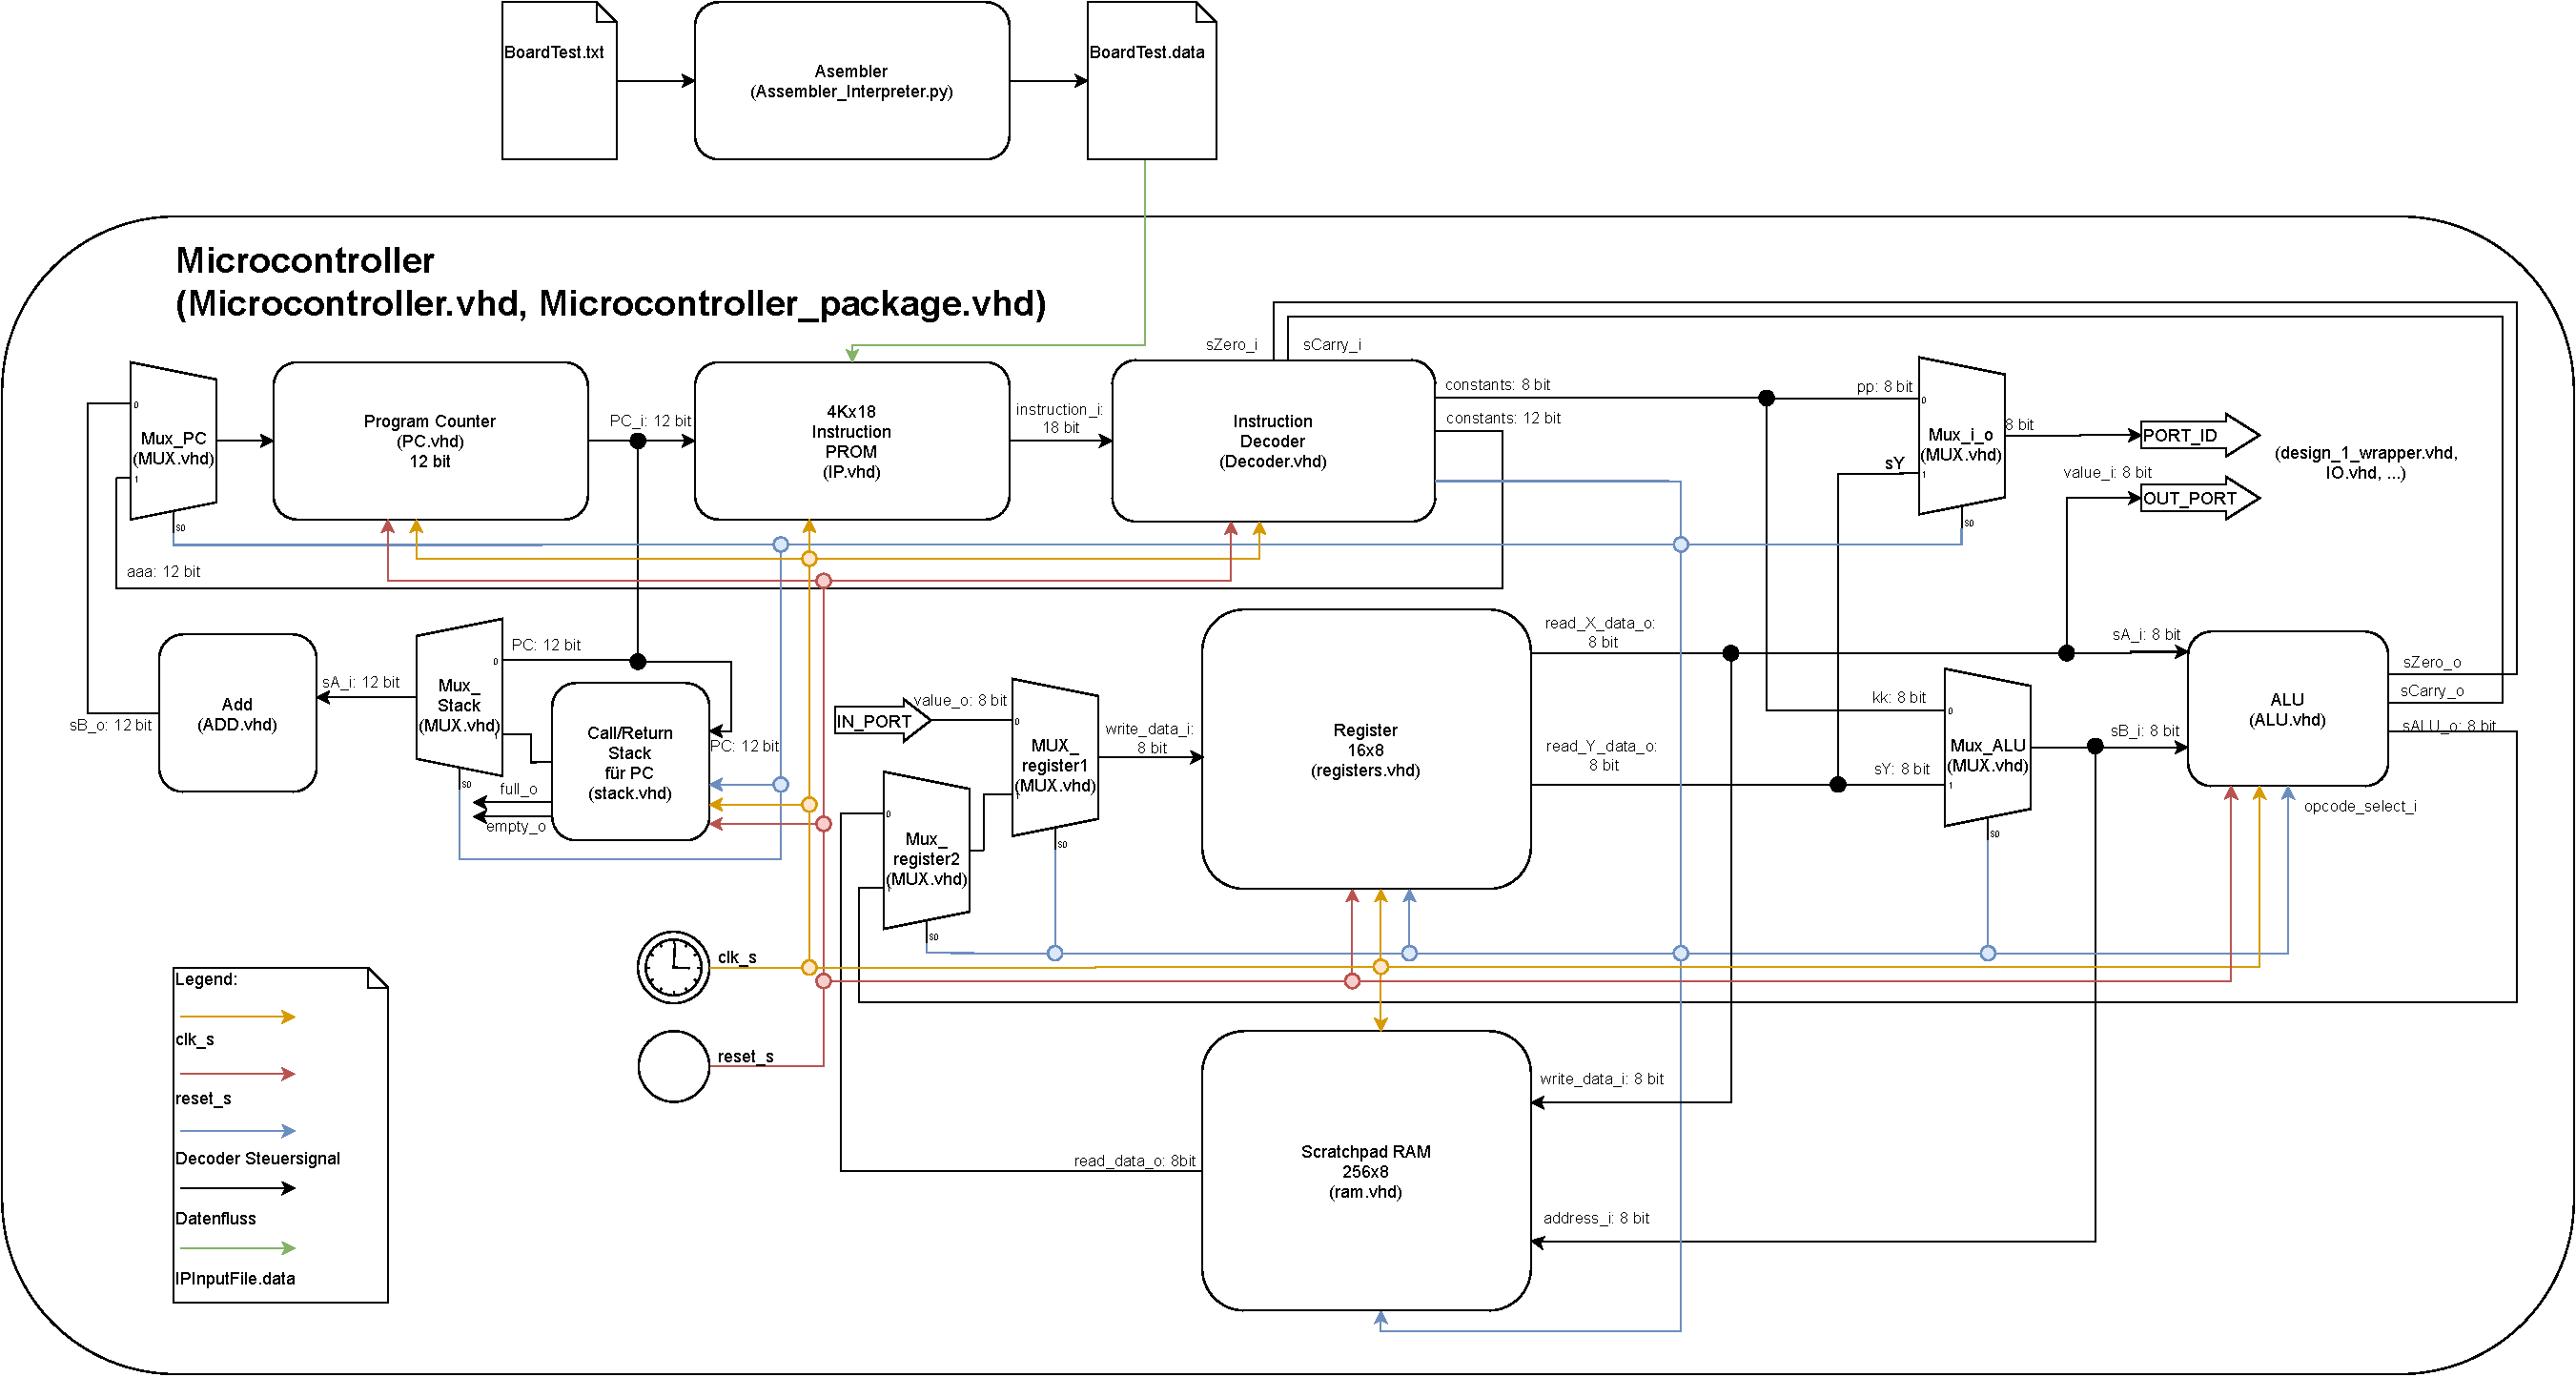
\includegraphics[width=\textwidth]{BlockdiagramMitVHDL.pdf}
    \caption{Top-Level Blockdiagramm des Mikroprozessors}
    \label{fig:toplevel_blockdiagramm}
\end{figure}
Die Abbildung zeigt die einzelnen Funktionsblöcke des Mikroprozessors, deren Verkabelung und Interaktionen sowie die Verknüpfung zum Assembler. Schwarze Pfade zeigen hierbei einen Datenfluss zwischen den Blöcken an, während die blauen Pfade Steuerbefehle des Instruction Decoders anzeigen. Alle Blöcke die eine Clock benötigen sind an die gelbe Leitung angeschlossen und alles was eine Reset-Funktion enthält an die rote Leitung.

\subsection{Blockbeschreibungen}
Im folgenden werden die einzelnen Funktionsblöcke des Mikroprozessors mit deren Ein-/Ausgänge, sowie deren Aufgabe innerhalb des Mikroprozessors beschrieben.


\subsubsection{Arithmetic Logic Unit (ALU)}
\begin{multicols}{2}
Hauptverantwortlich: Alexander Bunz, Omar Al Kadri, Simon Naß \\
Die ALU führt Operationen auf zwei Eingabedaten aus wenn das enable\_i Signal auf 1 gesetzt ist. Die Operationen umfassen Arithmetische, Logische Verknüpfungen und Shift Operationen. Die Eingabedaten sind entweder Konstante Werte vom Instruction Decoder (kk) oder aus den Registern (sX,sY) geladene Werte. Sie werden an den Eingängen sA\_i und sB\_i angelegt. Der opcode\_select\_i Eingang (vom Instruction Decoder), entscheidet darüber, welche Operation auf den Eingabedaten ausgeführt wird. Das Ergebnis der ausgeführten Operation wird an sALU\_o angelegt.
Die sZERO\_o und sCARRY\_o ausgänge werden je nach Operation, entsprechend der unten aufgeführten Tabelle (\ref{tab:1}), gesetzt.
\begin{figure}[H]
    \centering
    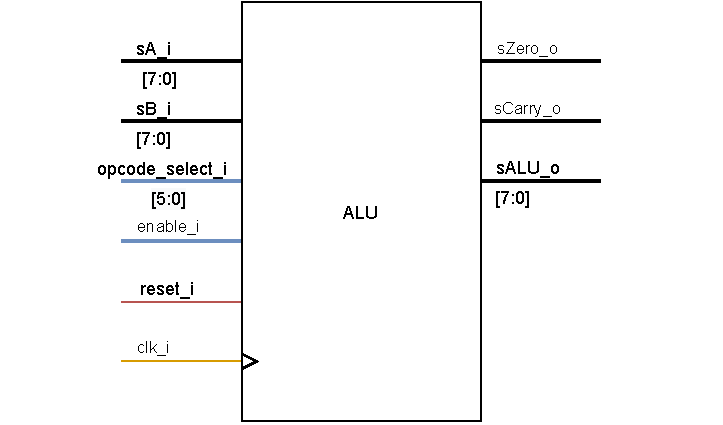
\includegraphics[width=0.5\textwidth]{ALU_beschreibung.pdf}
    \caption{Blockdiagramm der ALU}
    \label{fig:Block_ALU}
\end{figure}
\end{multicols}


\subsubsection{Instruction Decoder}
\begin{multicols}{2}
Hauptverantwortlich: Omar Al Kadri\\
Unterstützt von: Alexander Bunz, Simon Naß\\
Der Instruction Decoder (ID) dekodiert die aus dem Instruktionsspeicher geladenen Befehle und sendet entsprechende Steuersignale an die einzelnen Komponenten. Die Instruktionen, die vom ID verarbeitet werden, liegen am Eingang instruction\_i in form von 18 bit an. Je nach Instruktion, werden die Werte an den Ausgänge des ID entsprechend gesetzt. An sRegister\_X\_adresse\_o und sRegister\_Y\_adresse\_o werden die in den Instruktionen vorhandenen Register Adressen ausgegeben und ans Register weitergeleitet.
Enthält die Instruktion konstanten, so werden diese entsprechen an die Ausgänge constant\_kk\_o (8 bit) und const\_aaa\_o (12 bit) angelegt. Die mux\_... Ausgänge leiten entsprechend der eingegangenen Instruktion Steuerbits an verschiedene Multiplexer weiter. Der sALU\_select\_o Ausgang gibt den Opcode der Instruction an die ALU weiter. Die ...write\_or\_read\_o Ausgänge signalisieren, ob ein Wert geschrieben oder gelesen werden soll. Die sRegister\_write\_enable\_o, sALU\_enable\_o, sPC\_enable\_o, sStack\_enable\_o, sRAM\_write\_or\_read\_o und sRAM\_enable\_o Ausgänge, steuern den zugriff auf Register, ALU, Stack und RAM.
\begin{figure}[H]
    \centering
    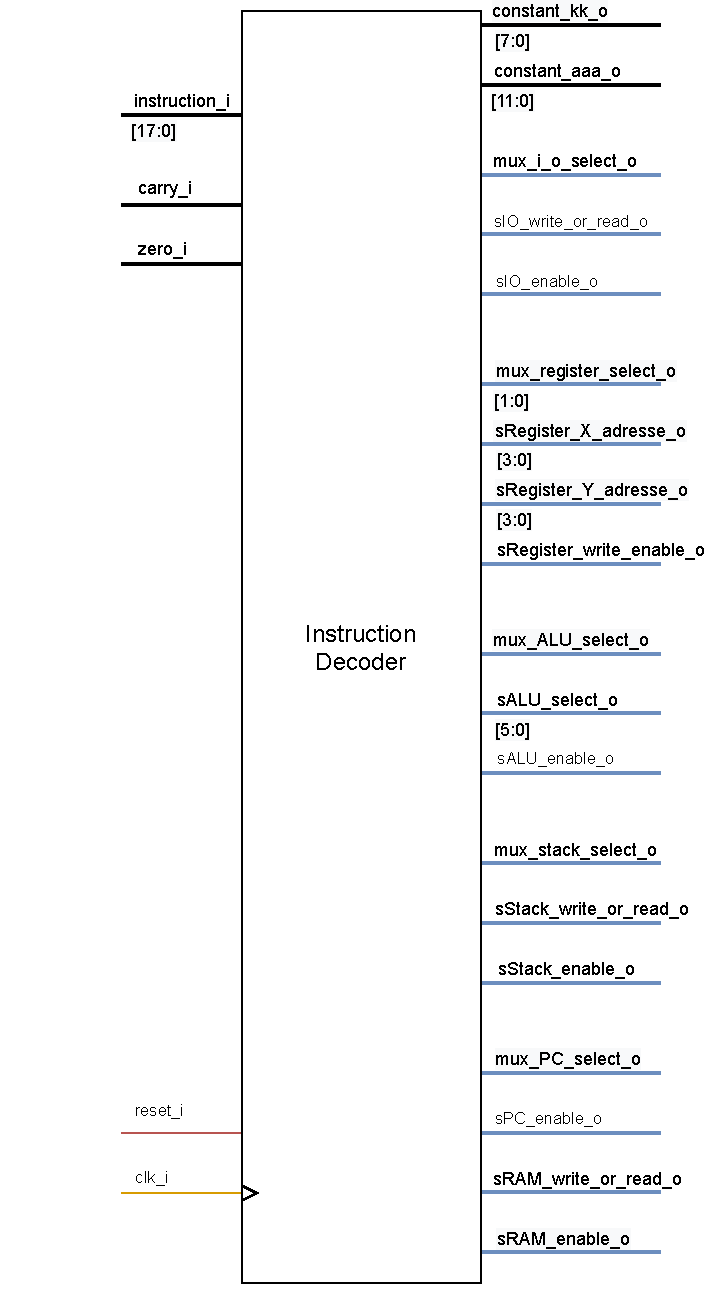
\includegraphics[height=0.5\textheight]{ID_beschreibung.pdf}
    \caption{Blockdiagramm des Instruction Decoders}
    \label{fig:Block_InstructionDecoder}
\end{figure}
\end{multicols}

\subsubsection{Program Counter}
\begin{multicols}{2}
Hauptverantwortlich: Jonas Unterweger\\
Unterstützt von: Simon Naß\\
Der Program Counter zeigt mit den Outputbits pc\_o auf die Position im Instruktionsspeicher, an welcher der aktuelle Befehl steht, der in den Instruktions Decoder geladen werden soll um ausgeführt zu werden. Bei jeder rising edge am clk\_i Input werden, falls das enable\_i Bit auf 1 gesetzt ist, die momentanen pc\_i Bits auf die pc\_o Bits übertragen, und damit der nächste Befehl geladen. \\
Durch ein setzten des reset\_i Bits auf 1 kann der Program Counter asynchron auf den ersten Befehl zurückgesetzt werden.
\begin{figure}[H]
    \centering
    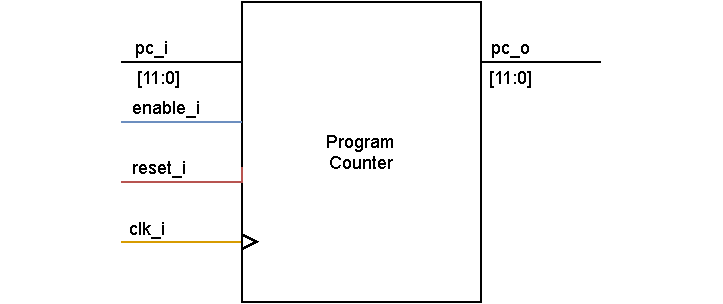
\includegraphics[width=0.5\textwidth]{ProgramCounter_beschreibung.pdf}
    \caption{Blockdiagramm des Program Counters}
    \label{fig:Block_ProgramCounter}
\end{figure}
\end{multicols}

\subsubsection{Scratchpad RAM}
\begin{multicols}{2}
Hauptverantwortlich: Jannik Graef\\
Unterstützt von: Tobias Weinschenk\\
Ein zusätzlicher Speicher um Werte zu Speichern. Das write\_or\_read\_i bit bestimmt ob gelesen oder geschrieben wird. Es wird entweder aus dem RAM die Daten an der Adresse address\_i auf read\_data\_o gelesen  oder es wird write\_data\_i auf die Adresse address\_i im RAM geschrieben. address\_i kommt entweder aus dem Register oder vom Instruction Decoder. write\_data\_i und read\_data\_o sind beide mit dem Register verbunden. Es wird nur aus dem RAM gelesen oder in den RAM geschrieben wenn enable\_i auf 1 gesetzt ist.
\begin{figure}[H]
    \centering
    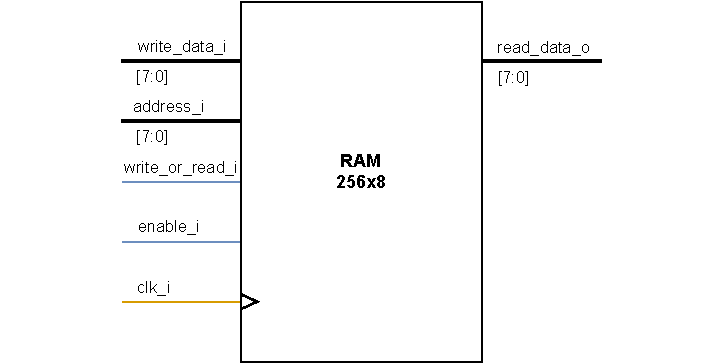
\includegraphics[width=0.5\textwidth]{RAM_beschreibung.pdf}
    \caption{Blockdiagramm des Scratchpad RAMs}
    \label{fig:Block_ScratchpadRAM}
\end{figure}
\end{multicols}

\subsubsection{Register}
\begin{multicols}{2}
Hauptverantwortlich: Tobias Weinschenk\\
Unterstützt von: Jannik Graef\\
Speichert 8bit Werte. Ergebnisse der ALU werden meist hierhin geschrieben. Das Register hat einen 8-bit breiten Eingang write\_data\_i um Daten anzunehmen, welche gespeichert werden sollen. Hierzu gibt es noch einen 4-bit breiten Eingang write\_address\_i um das Register auszuwählen und das write\_enable\_i bit um das schreiben zu aktivieren. Um aus dem Register zu lesen gibt es zwei Eingänge read\_X\_address\_i und read\_Y\_address\_i um die Register auszuwählen und zwei Ausgänge read\_X\_data\_o read\_Y\_data\_o auf welchen die Daten ausgegeben werden. So können zwei Werte aus dem Register gelesen werden. Über den reset\_i Eingang lässt sich das gesamte Register auf 0-Einträge zurücksetzen.
\begin{figure}[H]
    \centering
    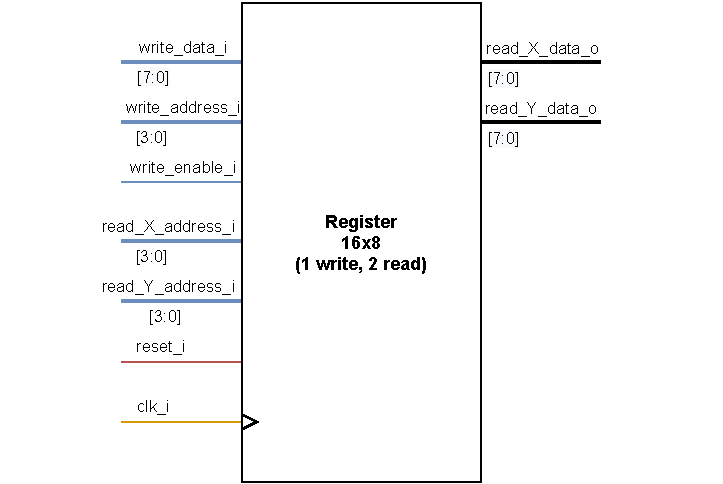
\includegraphics[width=0.5\textwidth]{Register_beschreibung.pdf}
    \caption{Blockdiagramm des Registers}
    \label{fig:Block_Register}
\end{figure}
\end{multicols}
\newpage
\subsubsection{Instruction Memory}
\begin{multicols}{2}
Hauptverantwortlich: Jochen Benzenhöfer\\
Ein Speicher in dem die Instruktionen als 18 Bit Werte gespeichert werden. Der Input(pc\_i) beschreibt die Stelle im Speicher, die derzeit ausgeführt wird und deshalb am Ausgang instruction\_o für den Instruction Decoder bereitliegt. Ändert sich der Input pc\_i ändert sich der Ausgang instruction\_o mit der nächsten steigenden Taktflanke von clk\_i.
\begin{figure}[H]
    \centering
    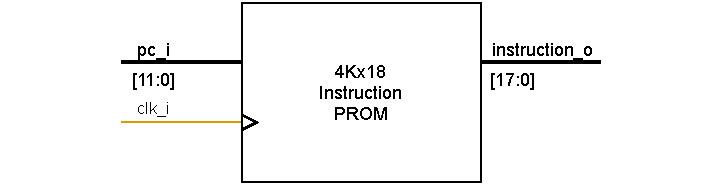
\includegraphics[width=0.5\textwidth]{IP_beschreibung.pdf}
    \caption{Blockdiagramm des Instruction PROM}
    \label{fig:Block_InstructionPROM}
\end{figure}
\end{multicols}

\subsubsection{CALL/RETURN Stack}
\begin{multicols}{2}
Hauptverantwortlich: Tobias Weinschenk\\
Ein Stackspeicher, der die Position des Program Counters vor einem Unterfunktionsaufruf speichert. Dabei werden die bei sPC\_i anliegenden Bits auf den Stack gespeichert, wenn write\_or\_read\_i auf 0 gesetzt ist, enable\_i auf 1 gesetzt ist und bei clk\_i ein rising edge vorliegt. Ist dagegen write\_or\_read\_i auf 1, werden bei der nächsten rising edge von clk\_i die oben auf dem Stack liegenden Bits auf den sStack\_o Output übertragen und vom Stack gelöscht. Ist enable\_i auf 0, so werden weder Daten auf den Stack gelegt, noch welche von ihm genommen. \\
Durch ein setzten von reset\_i auf 1 lässt sich der Stack asynchron resetten und damit leeren. \\
Über die Ausgänge full\_o und empty\_o zeigt der Stack, für full\_o = 1, dass er voll ist (somit werden weitere Schreibvorgänge verworfen) oder mit empty\_o = 1, dass er leer ist (somit werden weitere Lesevorgänge nicht ausgeführt).
\begin{figure}[H]
    \centering
    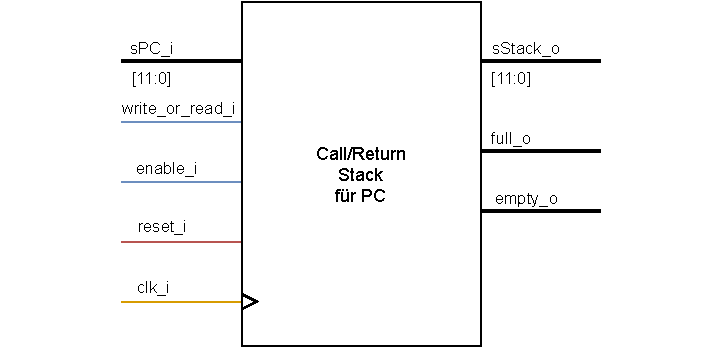
\includegraphics[width=0.5\textwidth]{Stack_beschreibung.pdf}\\
    \caption{Blockdiagramm des CALL/RETURN Stack}
    \label{fig:Block_Stack}
\end{figure}
\end{multicols}

\subsubsection{Input/Output}
\begin{multicols}{2}
Hauptverantwortlich: Jochen Benzenhöfer\\
Die nach außen zu sendenden Signale(erhalten durch value\_i) werden am Port mit der Nummer gegeben durch port\_id\_i ausgegeben, falls in\_out\_i und enable\_i den Wert 1 enthält. Falls enable\_i den Wert 1 und in\_out\_i 0 enthält, wird der derzeit anliegende Wert beim Port der port\_id\_i in value\_o gespeichert.
\begin{figure}[H]
    \centering
    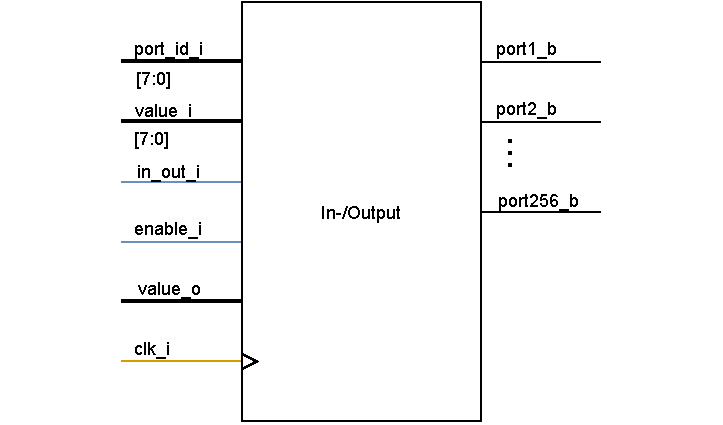
\includegraphics[width=0.5\textwidth]{IO_beschreibung.pdf}
    \caption{Blockdiagramm des Input/Output-Moduls}
    \label{fig:Block_IO}
\end{figure}
\end{multicols}

\newpage

\begin{small}
\begin{longtable}{||c|p{4cm}|p{10cm}||}
        \hline \hline
         Port & Beschreibung & Funktion  \endhead \caption{Portbelegung der Eingabeports} \endfoot \hline
         %44-46& Hdmi-Operationsauswahl & Wendet den Operator auf den Eingang(und die gegebenen Werte) an, legt den Wert am HDMI- Ausgang an.\newline
         %0- Addition(ohne Überlauf)\newline
         %1- Addition mod 256\newline
         %2- Subtraktion(ohne Überlauf)\newline
         %3- Subtraktion mod 256\newline
         %4- Multiplikation(ohne Überlauf)\newline
         %5- Multiplikation mod 256\newline
         %6- $\left\lceil\text{Division}\right\rceil$\newline
         %7- $\left\lfloor\text{Division}\right\rfloor$\newline
         %8- Logisches Und\newline
         %9- Logisches Oder\newline
         %10- Logisches XOR\newline
         %11- Negation\newline
         %12- Logisches Nand\newline
         %13- Logisches Nor\newline
         %14- Logisches XNor\newline
         %Rest- Ersetzen\newline
         %Port 44 für Blau, Port 45 für Grün und Port 46 für Rot\\\hline 
         %47-49 & Hdmi- Operationswert & Wert, der mit der gegebenen Operation auf den Eingangswert angewendet wird und am HDMI- Ausgang ausgegeben wird. Port 47 für Blau, Port 48 für Grün und Port 49 für Rot\\\hline
         50-53 & Pmod-Eingang & In dem jeweiligen Vektor stellen die Positionen jeweils einen Pin im Anschluss dar. Die verschiedenen Anschlüsse können durch die Portnummer angesprochen werden. Der Wert wird nur aktualisiert, wenn der jeweilige Port zuvor auf empfangen gesetzt wurde.\\\hline
         54 & Pmod-In-Out Schalter & Schaltet die Pmodgeräte als Eingang oder Ausgang. 0 Eingabe, 1 Ausgabe. Defaultwert: 0000\\\hline
         55 & Resetschalterauswahl auslesen & Defaultwert: 10000000; Gibt aus, welche Knöpfe/Schalter aktuell als reset benutzt werden können.\\\hline
         56-59 & alter Pmod-Eingang & In dem jeweiligen Vektor stellen die Positionen jeweils einen Pin im Anschluss dar. Die verschiedenen Anschlüsse können durch die Portnummer angesprochen werden. \\\hline
         60, 61 & Gibt die alte Belegung der Knöpfe und Schalter als Vektor aus & Schalter(0 bis 3) in Ausgabe(0 bis 3), Knöpfe(0 bis 3) in Ausgabe(4 bis 7). 61 letzte Belegung, 60 vorletzte Belegung.\\\hline
         62 & Gibt die aktuelle Belegung der Knöpfe und Schalter als Vektor aus & Schalter(0 bis 3) in Ausgabe(0 bis 3), Knöpfe(0 bis 3) in Ausgabe(4 bis 7).\\\hline
         63-255 & Port-Speicherzugriff & Unbenutzte Ports, welche als Speicher genutzt werden können- die Ausgabeports werden direkt auf die jeweiligen Eingabeports abgebildet. Liest den Speicher assoziiert mit dem Port aus und gibt den Inhalt aus.\\\hline
    \end{longtable}
    
    
    \begin{longtable}{||c|p{4cm}|p{10cm}||}
        \hline \hline
         Port & Beschreibung & Funktion  \endhead \caption{Portbelegung der Ausgabeports} \endfoot \hline
         %44-46 & Alte HDMI-Ausgabe & Gibt den RGB-Wert der vorherigen Hdmi-Eingabe aus. Port 44 für Blau, Port 45 für Grün und Port 46 für Rot\\\hline
         %47-49 & HDMI-Ausgabe & Gibt den RGB-Wert der Hdmi-Eingabe aus. Port 47 für Blau, Port 48 für Grün und Port 49 für Rot\\\hline
         50-53 & Pmod-Ausgang & In dem jeweiligen Vektor stellen die Positionen jeweils einen Pin im Anschluss dar. Die verschiedenen Anschlüsse können durch die Portnummer angesprochen werden. Ein Senden ist nur möglich, wenn der Port auf Senden gesetzt wurde.\\\hline
         54 & Pmod-In-Out Schalter Ausgabe & Gibt aus, ob die Pmodgeräte als Eingang oder Ausgang genutzt werden. 0 Eingabe, 1 Ausgabe. Defaultwert: 0000\\\hline
         55 & Resetschalterauswahl & Defaultwert: 10000000; Eingangswert xnor aktuellerWert = neuerWert, 1 bedeutet, das wenn dieser Knopf/ Schalter den Wert 1 sendet, ein reset signal gesendet wird.\\\hline
         56 - 62 & Ausgabe für LEDs & Port(56 bis 59) für LED 0 bis 4, Port(60 bis 62) für RGB von LED 5.\newline
        Die Eingabe stellt linear die Helligkeit der LED dar. 0 für aus, 255 für maximale Helligkeit.\\\hline
        63-255 & Port-Speicherschreiben & Unbenutzte Ports, welche als Speicher genutzt werden können- die Ausgabeports werden direkt auf die jeweiligen Eingabeports abgebildet. Schreibt in den Speicher assoziiert mit dem Port Eingabe.\\\hline
         
    \end{longtable}

\end{small}
\newpage
\subsection{Instruktionen}\label{sec:Instruktionen}

\begin{small}
    \begin{longtable}{||c|p{6.5cm}|c||}
        \hline \hline
         Instruktion & Beschreibung & Funktion  \endfirsthead
         \caption{Beschreibung und Funktion der Instruktionen}\\
         \hline \hline
         Instruktion & Beschreibung & Funktion \endhead \caption[]{Beschreibung und Funktion der Instruktionen}\endfoot
         \hline
         ADD sX, kk & Addiert zum Register sX das Literal kk hinzu. & sX $\leftarrow$ sX + kk  \\ \hline
         ADD sX, sY & Addiert zum Register sX den Inhalt aus Register sY hinzu. & sX $\leftarrow$ sX + sY   \\ \hline
         ADDCY sX, kk & Addiert zum Register sX das Literal kk mit Carry-Bit hinzu. &sX $\leftarrow$ sX+kk+CARRY   \\ \hline
         ADDCY sX, sY & Addiert zum Register sX den Inhalt aus Register sY mit Carry-Bit hinzu. & sX $\leftarrow$ sX+sY+CARRY  \\ \hline
         AND sX, kk & Bitweises UND von Register sX mit dem Literal kk. & sX $\leftarrow$ sX AND kk  \\ \hline
         AND sX, sY & Bitweises UND von Register sX mit Register sY. & sX $\leftarrow$ sX AND sY  \\ \hline
          CALL aaa & Bedingungsloser Aufruf der Unterfunktion an der Adresse aaa. &TOS $\leftarrow$ PC, PC $\leftarrow$ aaa  \\ \hline
         CALLC aaa & Falls CARRY-Bit gesetzt, Aufruf der Unterfunktion an der Adresse aaa. &if CARRY =1 {TOS $\leftarrow$ PC, PC $\leftarrow$ aaa}  \\ \hline
         CALLNC aaa & Falls CARRY-Bit nicht gesetzt, Aufruf der Unterfunktion an der Adresse aaa. &if CARRY =0 {TOS $\leftarrow$ PC, PC $\leftarrow$ aaa} \\ \hline
         CALLNZ aaa & Falls ZERO-Bit nicht gesetzt, Aufruf der Unterfunktion an der Adresse aaa. &if ZERO=0 {TOS $\leftarrow$ PC, PC $\leftarrow$ aaa}  \\ \hline
         CALLZ aaa & Falls ZERO-Bit gesetzt, Aufruf der Unterfunktion an der Adresse aaa. &if ZERO=1{TOS $\leftarrow$ PC, PC $\leftarrow$ aaa}\\ \hline
         COMPARE sX, kk & Vergleicht Register sX mit dem Literal kk. Setzt das CARRY und ZERO flag wie angegeben, Register bleiben dabei unverändert. & \makecell{if sX = kk ZERO $\leftarrow$ 1, \\ if sX \textless $ $ kk CARRY $\leftarrow$ 1 }  \\ \hline
         COMPARE sX, sY & Vergleicht Register sX mit dem Register sY. Setzt das CARRY und ZERO flag wie angegeben, Register bleiben dabei unverändert. & \makecell{sX = sY ZERO $\leftarrow$ 1, \\ if sX \textless $ $ sY CARRY $\leftarrow$ 1  }  \\ \hline
         FETCH sX, (sY) & Lese scratchpad RAM von der in Register sY gespeicherten Adresse in Register sX &sX $\leftarrow$ RAM[(sY)]   \\ \hline
         FETCH sX, ss & Lese scretchpad RAM von Adresse ss in Register sX &sX $\leftarrow$ RAM[ss]  \\ \hline
         INPUT sX, (sY) & Lese Wert des Input-Port, welcher vom Register sY spezifiziert wird, in das Register sX. &PORT\_ID $\leftarrow$ sY, sX $\leftarrow$ IN\_PORT  \\ \hline
         INPUT sX, pp & Lese Wert des Input-Port, welcher von pp spezifiziert wird, in das Register sX. &PORT\_ID $\leftarrow$ pp, sX $\leftarrow$ IN\_PORT \\ \hline
         JUMP aaa & Bedingungsloser Sprung nach aaa. &pc $\leftarrow$ aaa  \\ \hline
         JUMPC aaa & Falls das CARRY-Bit gesetzt ist, springe zu aaa. & if CARRY=1 pc $\leftarrow$ aaa \\ \hline
         JUMPNC aaa & Falls das CARRY-Bit nicht gesetzt ist, springe zu aaa. &if CARRY=0 pc $\leftarrow$ aaa  \\ \hline
         JUMPNZ aaa & Falls das ZERO-Bit nicht gesetzt ist, springe zu aaa. &if ZERO=0 pc $\leftarrow$ aaa  \\ \hline
         JUMPZ aaa & Falls das ZERO-Bit gesetzt ist, springe zu aaa. &if ZERO=1 pc $\leftarrow$ aaa  \\ \hline 
         LOAD sX, kk & Lade das Literal kk in das Register sX. &sX $\leftarrow$ kk   \\ \hline
         LOAD sX, sY & Lade den Inhalt des Registers sY in das Register sX. &sX $\leftarrow$ sY  \\ \hline 
         OR sX, kk & Bitweise OR von Register sX mit literal kk. &sX $\leftarrow$ sX OR kk   \\ \hline
         OR sX, sY & Bitweise OR von Register sX mit Register sY. & sX $\leftarrow$ sX OR sY   \\ \hline
         OUTPUT sX, (sY) & Schreibe Register sX zum in sY gespeicherten output Port. &PORT\_ID $\leftarrow$ sY, OUT\_PORT $\leftarrow$ sX  \\ \hline
         OUTPUT sX, pp & Schreibe Register sX zu output Port pp. &PORT\_ID $\leftarrow$ pp, OUT\_PORT $\leftarrow$ sX  \\ \hline
         RETURN & Bedingungslose Rückkehr von der Unterfunktion. & PC $\leftarrow$ TOS+1  \\ \hline
         RETURNC & Falls Carry-Bit gesetzt, Rückkehr von der Unterfunktion. & If CARRY=1, PC $\leftarrow$ TOS+1 \\ \hline
         RETURNNC & Falls Carry-Bit nicht gesetzt, Rückkehr von der Unterfunktion. & If CARRY=0, PC $\leftarrow$ TOS+1 \\ \hline
         RETURNZ & Falls Zero-Bit gesetzt, Rückkehr von der Unterfunktion.& If ZERO=1, PC $\leftarrow$ TOS+1 \\ \hline
         RETURNNZ & Falls Zero-Bit nicht gesetzt, Rückkehr von der Unterfunktion. & If ZERO=0, PC $\leftarrow$ TOS+1  \\ \hline
         RL sX & Rotiert Register sX einen Schritt nach links. &sX $\leftarrow$ {sX[6:0],sX[7]}, CARRY $\leftarrow$ sX[7]  \\ \hline
         RR sX & Rotiert Register sX einen Schritt nach rechts. &sX $\leftarrow$ {sX[0],sX[7:1]},CARRY $\leftarrow$ sX[0]   \\ \hline
         SL0 sX & Schiebe Register sX links, mit 0 aufgefüllt. &sX $\leftarrow$ {sX[6:0],0}, CARRY $\leftarrow$ sX[7]  \\ \hline
         SL1 sX & Schiebe Register sX links, mit 1 aufgefüllt. &sX $\leftarrow$ {sX[6:0],1}, CARRY $\leftarrow$ sX[7]  \\ \hline
         SLA sX & Schiebe Register sX links durch alle Bits, inklusive Carry. &sX $\leftarrow$ {sX[6:0],CARRY}, CARRY $\Leftarrow$ sX[7]  \\ \hline
         SLX sX & Schiebe Register sX links. Bit sX[0] unbetroffen. &sX $\leftarrow$ {sX[6:0],sX[0]}, CARRY $\leftarrow$ sX[7]  \\ \hline
         SR0 sX & Schiebe Register sX rechts, mit 0 aufgefüllt. &sX $\leftarrow$ {0,sX[7:1]}, CARRY $\leftarrow$ sX[0]  \\ \hline
         SR1 sX & Schiebe Register sX rechts, mit 1 aufgefüllt. &sX $\leftarrow$ {1,sX[7:1]}, CARRY $\leftarrow$ sX[0]  \\ \hline
         SRA sX & Schiebe Register sX durch alle bits, inklusive Carry. &sX $\leftarrow$ {CARRY,sX[7:1]}, CARRY $\leftarrow$ sX[0]  \\ \hline
         SRX sX & Arithmetisches rechtsschieben von Register sX mit Vorzeichenerweiterung. &sX $\leftarrow$ {s[7],sX[7:1]}, CARRY $\leftarrow$ sX[0]  \\ \hline
         STORE sX, (sY) & Schreibe Register sX in scratchpad RAM an der in Register sY gespeicherten Adresse. &RAM[(sY)] $\leftarrow$ sX \\ \hline
         STORE sX, ss & Schreibe Register sX an Adresse ss in scratchpad RAM. &RAM[ss] $\leftarrow$ sX \\ \hline
         SUB sX, kk & Subtrahiere literal kk von Register sX. &sX $\leftarrow$ sX-kk  \\ \hline
         SUB sX, sY & Subtrahiere Register sY von Register sX. &sX $\leftarrow$ sX-sY  \\ \hline
         SUBCY sX, kk & Subtrahiere literal kk von Register sX mit Carry. &sX $\leftarrow$ sX-kk-CARRY  \\ \hline
         SUBCY sX, sY & Subtrahiere Register sY von Register sX mit Carry. &sX $\leftarrow$ sX-sY-CARRY  \\ \hline
         TEST sX, kk & Teste Bits in Register sX gegen literal kk. Update Carry und Zero flags. Register bleiben unverändert. & \makecell{if(sX AND kk)=0 ZERO $\leftarrow$ 1, \\ CARRY $\leftarrow$ odd parity of (sX AND kk) }   \\ \hline
         TEST sX, sY  & Teste Bits in Register sX gegen Bits in Register sY. Update Carry und Zero flags. Register bleiben unverändert. & \makecell{if(sX AND sY)=0 ZERO $\leftarrow$ 1, \\ CARRY $\leftarrow$ odd parity of (sX AND sY) }  \\ \hline
         XOR sX, kk & Bitweise XOR von Register sX mit literal kk. &sX $\leftarrow$ sX XOR kk  \\ \hline
         XOR sX, sY & Bitweise XOR von Register sX mit Register sY. &sX $\leftarrow$ sX XOR sY   \\ \hline
    
    \end{longtable}
    %\captionof{table}{test}


\newpage
\begin{longtable}{||c|p{6cm}|p{6cm}|c||}
\hline \hline
    Instruktion & ZERO & CARRY & opcode\\    \endfirsthead
     \caption{Opcode Definition, sowie Carry + Zero-Flag Verhalten der Instruktionen}\\
     \hline \hline
     Instruktion & ZERO & CARRY & opcode\\ \endhead
     \caption[]{Opcode Definition, sowie Carry + Zero-Flag Verhalten der Instruktionen}\endfoot
    \hline
    ADD sX, kk & if (sX + kk = (0 or 256)): ZERO = 1,\newline else: ZERO = 0
    & if ((sX + kk) $>$ 255): CARRY = 1,\newline else: CARRY = 0 & 000001 \\ \hline
    ADD sX, sY & if (sX + sY = (0 or 256)): ZERO = 1,\newline else: ZERO = 0
    & if ((sX + sY) $>$ 255): CARRY = 1,\newline else: CARRY = 0 & 000000 \\ \hline
    ADDCY sX, kk & if (sX + kk + CARRY = (0 or 256)): ZERO = 1,\newline else: ZERO = 0
    & if ((sX + kk + CARRY) $>$ 255): CARRY = 1,\newline else: CARRY = 0 & 000011 \\ \hline
    ADDCY sX, sY & if (sX + sY + CARRY = (0 or 256)): ZERO = 1,\newline else: ZERO = 0
    & if ((sX + sY + CARRY) $>$ 255): CARRY = 1,\newline else: CARRY = 0 & 000010 \\ \hline
    AND sX, kk & if (sX AND kk = 0): ZERO = 1,\newline else: ZERO = 0 & 0 & 001001 \\ \hline
    AND sX, sY & if (sX AND sY= 0): ZERO = 1,\newline else: ZERO = 0 & 0 & 001000 \\ \hline
    CALL aaa & - & - & 100001 \\ \hline
    CALLC aaa  & - & - & 100010 \\ \hline
    CALLNC aaa & - & - & 100011 \\ \hline
    CALLNZ aaa & - & - & 100100 \\ \hline
    CALLZ aaa & - & - & 100101 \\ \hline
    COMPARE sX, kk & if (sX = kk): ZERO = 1,\newline else: ZERO = 0
    & if (kk $>$ sX): CARRY = 1,\newline else: CARRY = 0 & 011011 \\ \hline
    COMPARE sX, sY & if (sX = sY): ZERO = 1,\newline else: ZERO = 0
    & if (sY $>$ sX): CARRY = 1,\newline else: CARRY = 0 & 011010 \\ \hline
    FETCH sX, (sY) & - & - & 010010 \\ \hline
    FETCH sX, ss & - & - & 010011 \\ \hline
    INPUT sX, (sY) & - & - & 010110 \\ \hline
    INPUT sX, pp & - & - & 010111 \\ \hline
    JUMP aaa & - & - & 100110 \\ \hline
    JUMPC aaa & - & - & 100111 \\ \hline
    JUMPNC aaa & - & - & 101000 \\ \hline
    JUMPNZ aaa & - & - & 101001 \\ \hline
    JUMPZ aaa & - & - & 101010 \\ \hline 
    LOAD sX, kk & - & - & 001111 \\ \hline
    LOAD sX, sY & - & - & 001110 \\ \hline 
    OR sX, kk & if (sX OR kk = 0): ZERO = 1,\newline else: ZERO = 0 & 0 & 001011 \\ \hline
    OR sX, sY & if (sX OR sY= 0): ZERO = 1,\newline else: ZERO = 0 & 0 & 001010 \\ \hline
    OUTPUT sX, (sY) & - & - & 010100 \\ \hline
    OUTPUT sX, pp & - & - & 010101 \\ \hline
    RETURN & - & - & 101011 \\ \hline
    RETURNC & - & - & 101100 \\ \hline
    RETURNNC & - & - & 101101 \\ \hline
    RETURNZ & - & - & 101110 \\ \hline
    RETURNNZ & - & - & 101111 \\ \hline
    RL sX & if (rl(sX) = 0): ZERO = 1,\newline else: ZERO = 0
    & CARRY = sX[7] & 110000 \\ \hline
    RR sX & if (rr(sX) = 0): ZERO = 1,\newline else: ZERO = 0
    & CARRY = sX[0] & 110001 \\ \hline
    SL0 sX & if (sl0(sX) = 0): ZERO = 1,\newline else: ZERO = 0
    & CARRY = sX[7] & 110010 \\ \hline
    SL1 sX & if (sl1(sX) = 0): ZERO = 1,\newline else: ZERO = 0
    & CARRY = sX[7] & 110011 \\ \hline
    SLA sX & if (sla(sX) = 0): ZERO = 1,\newline else: ZERO = 0
    & CARRY = sX[7] & 110100 \\ \hline
    SLX sX & if (slx(sX) = 0): ZERO = 1,\newline else: ZERO = 0
    & CARRY = sX[7] & 110101 \\ \hline
    SR0 sX & if (sr0(sX) = 0): ZERO = 1,\newline else: ZERO = 0
    & CARRY = sX[0] & 110111 \\ \hline
    SR1 sX & if (sr1(sX) = 0): ZERO = 1,\newline else: ZERO = 0
    & CARRY = sX[0] & 110111 \\ \hline
    SRA sX & if (sra(sX) = 0): ZERO = 1,\newline else: ZERO = 0
    & CARRY = sX[0] & 111000 \\ \hline
    SRX sX & if (srx(sX) = 0): ZERO = 1,\newline else: ZERO = 0
    & CARRY = sX[0] & 111001 \\ \hline
    STORE sX, (sY) & - & - & 010000 \\ \hline
    STORE sX, ss & - & - & 010001 \\ \hline
    SUB sX, kk & if ((sX - kk) = 0): ZERO = 1,\newline else: ZERO = 0
    & if ((sX - kk) $<$ 0): CARRY = 1,\newline else: CARRY = 0 & 000101 \\ \hline
    SUB sX, sY & if ((sX - sY) = 0): ZERO = 1,\newline else: ZERO = 0
    & if ((sX - sY) $<$ 0): CARRY = 1,\newline else: CARRY = 0 & 000100 \\ \hline
    SUBCY sX, kk & if ((sX - kk- CARRY) = (0 or -256): ZERO = 1,\newline else: ZERO = 0
    & if ((sX - kk - CARRY) $<$ 0): CARRY = 1,\newline else: CARRY = 0 & 000111 \\ \hline
    SUBCY sX, sY & if ((sX - sY - CARRY) = (0 or -256): ZERO = 1,\newline else: ZERO = 0
    & if ((sX - sY - CARRY) $<$ 0): CARRY = 1,\newline else: CARRY = 0 & 000110 \\ \hline
    TEST sX, kk & if (sX AND kk = 0): ZERO = 1,\newline else: ZERO = 0
    & if (parityTest\footnote{parityTest() testet, ob die Eingabe eine gerade oder ungerade Anzahl an '1'bit besitzt.}(sX And kk) = 1): CARRY = 1,\newline else: CARRY = 0 & 011001 \\ \hline
    TEST sX, sY  & if (sX AND sY = 0): ZERO = 1,\newline else: ZERO = 0
    & if (parityTest\footnotemark[1](sX And sY) = 1): CARRY = 1,\newline else: CARRY = 0 & 011000 \\ \hline
    XOR sX, kk & if (sX XOR kk = 0): ZERO = 1,\newline else: ZERO = 0 & 0 & 001101 \\ \hline
    XOR sX, sY & if (sX XOR sY = 0): ZERO = 1,\newline else: ZERO = 0 & 0 & 001100 \\ \hline
\end{longtable}
\label{tab:1}

\end{small}
\newpage
\section{Entwicklungsprozess}\label{sec:Entwicklungsprozess}%Schwierigkeiten und deren Lösung

\subsection{ALU}
Hauptverantwortlich: Alexander Bunz, Omar Al Kadri, Simon Naß.\\\\
In der ALU wurde zu beginn die Shiftbefehle, umgesetzt diese haben wie bereits hier schon in ersten Tests ersichtlich, keine Fehler. \\
Als nächstes wurden Logikbefehle implementiert. Aufgrund von unklarer Dokumentation des Zero und Cary Signals, traten hier Unterschiede zwischen dem Testergebnis und dem erwarteten Ergebnis auf. Nach Anpassung im ALU Code traten keine weiteren Fehler bezüglich Logikbefehlen auf. Es ist jedoch anzumerken, dass die Dokumentation diesbezüglich nach den ausführlichen externen Tests zur deutlicheren Klarstellung überarbeitet wurde. \\
Bei den arithmetischen Befehlen wurden Zweifel an der fehlerfreien Funktionsweise auf dem Bord geäußert, wodurch sie auf unterschiedlichste Weise zusätzlichen Prüfungen unterzogen wurden. Es konnten jedoch keine Nachteile dieser Implementierungsweise festgestellt werden. Bei den ausführlichen externen Tests trat ein Fehler bei der Operation SUBCY auf. Hier konnte durch einen Overflow das CARRY nicht richtig ermittelt werden. 
\begin{small}
\begin{minted}[tabsize=2,breaklines]{vhdl}
when operation_SUBCY | operation_SUBCY_kk=>
	result_s <= to_stdulogicvector(to_stdlogicvector(sA_i) - to_stdlogicvector(sB_i) - carry_s);
	if (to_stdlogicvector(sA_i) < (to_stdlogicvector(sB_i) + carry_s)) then 
		carry_s <= '1';
	else
		carry_s <= '0';
	end if;
\end{minted}
\end{small}
Vorheriger Code zeigt die Umsetzung des fehlerhaften Bereich vor Problembehebung in der ALU. Die Korrektur ist im folgenden Codeausschnit dargestellt.\\
\begin{small}
\begin{minted}[tabsize=2,breaklines]{vhdl}
when operation_SUBCY | operation_SUBCY_kk=>
	result_s <= to_stdulogicvector(to_stdlogicvector(sA_i) - to_stdlogicvector(sB_i) - carry_s);
	if (('1'&to_stdlogicvector(sA_i))-carry_s) < ('1'&to_stdlogicvector(sB_i))  then 
		carry_s <= '1';
	else
		carry_s <= '0';
	end if;
\end{minted}
\end{small}

\subsection{Instruction Decoder}
Hauptverantwortlich: Omar Al Kadri.\\
Unterstützt von: Alexander Bunz und Simon Naß.\\\\
Der Instruction Decoder wurde zunächst vollständig innerhalb eines Prozesses implementiert, um je nach Befehl entsprechende Steuersignale abhängig vom Takt zu setzen. Dies erwies sich allerdings aus zweierlei Hinsicht als unvorteilhaft. Zum Einen wurde der Decoder durch viele switch cases sehr groß und unübersichtlich, zum anderen konnten die Enable Signale für die anderen Komponenten nicht in einer bestimmten zeitlichen Abfolge gesetzt werden. \\
Deshalb haben wir den Decoder so umstrukturiert, dass die einzelnen Enable Signale über eine State Machine gesteuert werden, sodass jeder Block einen Takt Zeit für seine Aufgaben hat. Dadurch wird gewährleistet, dass jeder Block genügend Zeit für seine Berechnungen hat und die Signale für andere Blöcke stabil anliegen. Damit gibt der Decoder auch die Zeit für die Abarbeitung einzelner Befehle vor. Jumps, Calls und Return Befehle benötigen vier Takt Zyklen und alle anderen Befehle benötigen sechs Takt Zyklen. \\
Das eigentliche Decodieren der Befehle wurde aus dem Prozess heraus verlagert und deutlich vereinfacht. Das Decodieren der Befehle geschieht nun unabhängig vom Takt, dem Decoder wird allerdings von der eigenen State Machine auch ein Takt Zeit dafür gegeben. \\
Beim Decoder wurden Instruktionen, die es eigentlich nicht gibt (wie z.B. "111111111111111111") zugelassen, da diese eigentlich durch das Assembler Programm gar nicht erst erzeugt werden können. Da solche Befehle dadurch allerdings unvorhergesehenen Einfluss auf ein Programm haben können und wir sicherstellen wollten, dass auch Maschinencode der nicht von unserem Assembler Programm erzeugt wird auf dem Prozessor laufen kann, haben wir uns am Ende noch dazu entschieden den Decoder so anzupassen, dass unbekannte Instruktionen einfach ignoriert werden. \\
Zuletzt hatten wir noch versucht einen Takt einzusparen, indem wir die Zustände der State Machine von dem Program Counter und dem Instruction PROM zu einem zusammenfassen und den ROM asynchron lesen. Dadurch konnte der Instruction PROM allerdings nicht mehr den Block-RAM des Boards verwenden, weshalb wir dies rückgängig gemacht haben.

\subsection{Program Counter}
Hauptverantwortlich: Jonas Unterweger.\\
Unterstützt von: Simon Naß.\\\\
Der Program Counter durchlief keine Änderungen, allerdings entstand durch seinen \glqq enable\_i\grqq \space Eingang in Zusammenarbeit mit dem Decoder eine allgemein wichtige Diskussion welche Blöcke ebenfalls ein \glqq enable\_i\grqq \space benötigen und wie der Decoder diese steuern soll.\\
Die relativ späte Implementierung der ADD-Komponente erwies sich als entsprechend einfach. Hier hat man nämlich auf die bereits in der ALU verwendete und getestete Variante gesetzt. Man hat sich jedoch von zwei auf einen Eingang um-entschieden, da man immer um demselben konstanten Wert ('1') inkrementieren wollte. Die ausführlichen externen Tests zeigten keine auffälligen oder fehlerhafte Verhalten. Das Anlegen eines undefinierten Signals führt natürlich in der Simulation zu einer Ungewissheit des Ausgangs, jedoch wird durch andere Komponenten sichergestellt, dass ein solches Signal hier niemals anliegen kann.

\subsection{Scratchpad RAM}
Hauptverantwortlich: Jannik Graef.\\  Unterstützt von: Tobias Weinschenk.\\\\
Die erste Idee war es den Inhalt des RAM als einzelnen, großen  std\_ulogic\_vector der Größe 2048 bit zu implementieren und immer Zugriff auf 8-bit Abschnitte zu gewähren.\\
\begin{small}
\begin{minted}[tabsize=2,breaklines]{vhdl}
signal data  : std_ulogic_vector(2047 downto 0);
...
if (clk_i'event and clk_i = '1' and  enable_i = '1') then
	address := to_integer(unsigned(address_i));
	if(write_or_read_i = '0') then
		read_data_o <= data((address+1)*ram_width_g-1 downto address*ram_width_g);
	else
		data((address+1)*ram_width_g-1 downto address*ram_width_g) <= write_data_i;
	end if;
end if;
\end{minted}
\end{small}
Es erwies sich jedoch als praktischer die Daten in einem eigenen Type zu speichern. Der definierte Type besteht aus einem 256 Elemente langem Array aus u\_logic\_vetor der Größe 8:\\
\begin{small}
\begin{minted}[tabsize=2,breaklines]{vhdl}
type ram_type is array (2 ** ram_select_size_g -1 downto 0) of std_ulogic_vector(ram_width_g -1 downto 0);
signal ram_s : ram_type := (others => (others => '0'));
...
if (rising_edge(clk_i) and  enable_i = '1') then
                if(write_or_read_i = '1') then
                    read_data_o <= ram_s(to_integer(unsigned(address_i)));
                else
                    ram_s(to_integer(unsigned(address_i))) <= write_data_i;
                end if;
            end if;
\end{minted}
\end{small}
Wie im gezeigten Code schon ersichtlich wurde der RAM zudem mit Generics versehen, um die Größe schnell anpassen zu können. Hierzu gibt es zwei Generics um die Größe zu steuern: \glqq ram\_witdh\_g \grqq \space gibt die Wortbreite des RAMs an, \glqq ram\_select\_size\_g \grqq \space gibt die Anzahl an Addressierungs-bits an. Das Array bekommt dann die Größe $2^{ram\_select\_size\_g}$.

Zudem wurde das Attribut \glqq ram\_style \grqq \space hinzugefügt, welches Vivado anweist einen bestimmten RAM-Typ zu synthetisieren. Zur Auswahl stehen, \glqq registers \grqq (Flip-Flops), \glqq distributed \grqq(Look-Up-Table RAM), sowie \glqq block \grqq (Block-RAM). Auch dieses Attribut kann per Generic schnell verändert werden. Am sinnvollsten scheint uns aber \glqq distributed \grqq, da Block-RAM nur in 32kB Blöcken verfügbar ist und somit mit den 2kB RAM kaum sinnvoll ausgelastet wird und auf der anderen Seite werden mit \glqq registers \grqq \space unnötig viele Flip-Flops verbraucht werden. Der LUT-RAM scheint daher angebracht. Im Testbench haben sich bei dieser Architektur keine Fehler gezeigt.

\subsection{Register}
Hauptverantwortlich: Tobias Weinschenk.\\ Unterstützt von: Jannik Graef.   \\\\

Da das Register in Zusammenarbeit mit dem RAM entstand, wurden hier die selben Überlegungen wie beim RAM angestellt. Auch hier war die Überlegung zunächst den gesamten Inhalt in einem Signal der Größe 128 bit zu speichern, welche schnell durch den eignen Type ersetzt wurde.
\begin{small}
\begin{minted}[tabsize=2,breaklines]{vhdl}
 type register_type is array (2 ** register_select_size_g -1 downto 0) of std_ulogic_vector(register_width_g -1 downto 0);
signal register_s : register_type := (others => (others => '0'));
...
if (reset_i = '1') then
                    register_s <= (others => (others => '0'));
                    read_X_data_o <= (others => '0');
                    read_Y_data_o <= (others => '0');
                elsif (rising_edge(clk_i)) then
                    read_X_data_o <= register_s(to_integer(unsigned(read_X_address_i)));
                    read_Y_data_o <= register_s(to_integer(unsigned(read_Y_address_i)));
                    if(write_enable_i = '1') then
                        register_s(to_integer(unsigned(write_address_i))) <= write_data_i;
                    end if;
                end if;
\end{minted}
\end{small}
Wie im Code ersichtlich, ist der Prozess des Registers, aufgrund der anderen Anforderungen, etwas anders aufgebaut. Zunächst, gibt es beim Register einen asynchronen Reset, welcher auch die Inhalte des Registers zurücksetzt. Außerdem gibt es zwei Ausgabeports, welche gleichzeitig gelesen werden können. Aber auch wie beim RAM wurde die Größe über die Generics \glqq register\_widt\_g \grqq  \space (Wort-Breite) und \glqq register\_select\_size\_g \grqq \space (Anzahl Addressierungs-bits) gesetzt. Durch den vorhandenen asynchronen Reset, viel die Überlegung, welcher Speichertyp verwendet werden soll hier allerdings weg, da hierdurch nur noch Flip-Flops verwendet werden können. Was aber auch sehr gut zum Aufgabenbereich und der Größe des Moduls passt. Auch hier haben sich in ausführlichen externen Tests keine Fehler gezeigt.

\subsection{Instruction Memory}
Hauptverantwortlich: Jochen Benzenhöfer.\\\\
Die erste Idee, das Programm für den Prozessor auf dem NOR-Speicher des Boards oder einer SD-Karte abzulegen und von dort aufzurufen klingt im ersten Moment sehr verlockend. Nach etwas Recherche stellte sich jedoch heraus, dass diese Speichermethoden nicht wirklich trivial sind. So lässt der NOR-Speicher nur über das PS (Processing System) auslesen und die SD-Karte liefert nur sehr langsam Daten. \\
Zur Umsetzung müsste somit ein RAM-Speicher als Zwischenspeicher erstellt werden. Deshalb wurde der Speicher komplett durch BRAM umgesetzt. Dieser ist auf dem Board ausreichend verfügbar, muss jedoch auch bei der Synthese initialisiert werden. Grundsätzlich wäre es auch möglich den PROM durch DRAM zu implementieren, durch die große Größe schien dies jedoch nicht wirklich praktikabel. Die Befürchtung, dass die Verzögerung durch Nutzung des BRAMs zu hoch sein könnte konnte in der Praxis nicht bestätigt werden, weshalb kein Cache zur Unterstützung vollständig implementiert wurde. \\
Die ausführlichen externen Tests ergaben, dass keine Fehler durch die Implementierung des Instruction Memorys mit dem BRAM auftreten. Kritisch ist jedoch der Inhalt der in das Instruction Memorys geladen werden kann. Hier sind sowohl im Assembler als auch im Instruction Decoder Maßnahmen vorhanden um einen fehlerhaften Kontrollfluss und unbekannte Instruktionen abzufangen. 

\subsection{Call/Return Stack}
Hauptverantwortlich: Tobias Weinschenk. \\
% implementation mit variablen
% probleme beim post-syntesis test, aber nicht aufgrund der variblen, sondern std_ulogic

Bei der Entwicklung des Stacks erwiesen sich die gewonnenen Kenntnisse über die unterschiedlichen Speicherarten und die Definition eines eigenen Types aus der Entwicklung des RAMs als sehr nützlich und wurden direkt umgesetzt. Da der Stack eine Tiefe von 128 besitzt und 12 Bits pro Eintrag Speichern soll, haben wir uns aufgrund der Speichermenge von 1,5 KiB  auch hier für den LUT-RAM entschieden. Aber auch beim Stack lässt sich der verwendete RAM-Typ, sowie die Wort-Breite als auch die Tiefe per Generics schnell ändern. \\
Die Funktionsweise des Stacks wurde komplett in einem Prozess unter der Verwendung von Variablen für den Stack-Pointer, dem Empty-Bit und dem Full-Bit umgesetzt. Allerdings sind beim ersten Test zwei Probleme aufgefallen. Das erste Problem war der Stack-Pointer, welcher die untere Ebene im Stack nie beschrieben hat. Dies kam dadurch zustande, dass der Stack-Pointer auf 0 initialisiert wird und vor jedem Schreiben um eins inkrementiert wird. Dadurch konnte die Ebene 0 nie beschreiben werden. Dies konnte durch eine Verschiebung bei der Definition des Arrays behoben werden. Somit wurde aus der Zeile:
\begin{small}
\begin{minted}[tabsize=2,breaklines]{vhdl}
type stack_type is array (stack_depth_g -1 downto 0) of std_ulogic_vector( instruction_address_g -1 downto 0);
\end{minted}
\end{small}
folgende Zeile:
\begin{small}
\begin{minted}[tabsize=2,breaklines]{vhdl}
type stack_type is array (stack_depth_g downto 1) of std_ulogic_vector( instruction_address_g -1 downto 0);
\end{minted}
\end{small}
 Beim zweiten Problem handelte es sich um den asynchronen Reset, da dieser zunächst auch den gesamten Inhalt des Stacks zurücksetzen sollte. Dies ist allerdings beim LUT-RAM, sowie Block-Ram nicht möglich. Daher haben wir uns entschieden, beim asynchronen Reset den Inhalt des Stacks nicht zu löschen, da es bereits ausreicht, den Stack-Pointer, sowie den Ausgang, das Empty-Flag und das Full-Flag zurückzusetzen. Ein Lesen bevor etwas geschrieben wird, ist aufgrund der Logik innerhalb des Prozesses nicht möglich. \\
 Weiterhin gab es noch Diskussionen über die Implementierung per Variablen. Es stellte sich die Frage, ob diese Implementierung sich auch nach der Synthese korrekt verhält. Hierbei gab es aber erneut Probleme. Der erstellte Testbench verwendet wie der Stack selbst den Datentyp std\_ulogic, allerdings wandelt Vivado den Stack bei der Synthese in den Datentyp std\_logic um, weshalb Vivado eine Fehlermeldung bezüglich der nicht übereinstimmenden Datentypen erzeugte. Dies konnte durch umschreiben des Testbenches auf den Datentyp std\_logic behoben werden. Hier zeigte sich nun auch, dass die Implementierung mit Variablen für den Stack-Pointer, sowie die Flags sich auch nach der Synthese verhält wie erwartet.
\\ \\
Ausführlichen externen Tests des Stacks ergaben eine fehlerfreie normaldurchlauf. Gerade das auslesen auf leerem Stack und schreiben auf vollem Stack sind interesante Randfälle. Betrachtet man das verhalten hier im Stack als alleinstehenden Block, so tut dieser das bestmögliche mit seinen \glqq full\_o\grqq und \glqq empty\_o\grqq Ausgangssignalen, sowie internen Stack verhalten. Allerdings wird zur derzeitigen Lage keine Fehlerbehandlung dieser Randfälle auf dem Board durchgeführt. Dies erfordert also eigene Aufmerksamkeit bei dem Programmieren der auf dem Board laufenden Programme. \\
Der vom Stack ausgegebene Resetwert war zwar in sich logisch wurde jedoch auf \glqq 111111111111\grqq abgeändert um im Gesamtkonzept mit dem Resetwert des Program Counters übereinzustimmen.

\subsection{Input/Output}
Hauptverantwortlich: Jochen Benzenhöfer.\\\\
Der einfachste Weg den Block umzusetzen wäre, die Daten durch die gegebene Port\_id zu den Prozessorpins zu multiplexen, jedoch fallen durch dieses System viele Probleme an.
\begin{enumerate}
    \item 
    Die Port\_id ist eine 8-Bit Zahl, wodurch bis zu 256 verschiedene Ports adressiert werden könnten, der Prozessor hat jedoch nur 230 Pins, welche jedoch nicht alle durch den FPGA-Teil direkt erreichbar sind. Somit musste ein Verhalten des Blocks bei unbenutzter Port\_id definiert werden, oder die unbenutzten Ports anderweitig verwendet werden.
    \item
    Der Prozessor geht davon aus, dass jeder Port bidirektional verfügbar ist. Dies ist jedoch nicht für jeden Pin der Fall, wodurch verschiedene Pins zu einem Port verbunden werden müssen, was 1. verstärkt. Eine weitere Lösung wäre, die ungenutzten unidirektionalen Ports anderweitig zu nutzen. Dies zerstört jedoch die einfache Multiplexerstruktur. Dieses Problem sorgte für weitere Probleme, da manche Pins (z.B. die HDMI-Pins) nicht durch einen inout Bus nutzbar sind. Es müssen somit mehrere Ein/Ausgangsvektoren zu den Pins verbunden werden.
    \item
    Jeder Pin kann nur mit einem Bit gleichzeitig benutzt werden. Die Eingabe- und Ausgabevektoren haben jedoch eine Größe von 8Bit. Gelöst werden kann dieses Problem entweder durch das nutzen mehrerer Pins gleichzeitig oder durch Serielle Nutzung der Pins. Die Parallele Nutzung ist oftmals nicht besonders sinnvoll, da hierdurch häufig verschiedene Geräte gleichzeitig benutzt werden. Bei der seriellen Nutzung muss die vom jeweiligen Protokoll genutzte Clock beachtet werden, was die Komplexität stark erhöht.
    \item
    Die verschiedenen Protokolle der Geräte benötigen synchron Daten auf verschiedenen Kanälen oder bestimmte Bitfolgen oder bestimmte Verschlüsselungen. Mit diesen Protokollen lässt sich mit einem Primitiven Multiplexer in Kombination mit unserem Prozessorinterface nur sehr schwer oder nicht kommunizieren.
    \item
    Ein- und Ausgaben müssen aktiv auf Veränderungen überprüft werden bzw. Verändert werden. Um z.B. eine LED nicht mit voller Helligkeit leuchten zu lassen muss diese an und ausgeschaltet werden. Dieses Problem kann durch Zwischenspeichern der Ein- und Ausgaben behoben werden. Ein weiterer Vorteil der Speicher ist, dass asynchrone Ein- und Ausgaben korrekt empfangen und gesendet werden können.
\end{enumerate}
Aufgrund dieser Probleme wurde das Portsytem verändert: Jeder Port hat eine Funktion angepasst an das jeweils verwendete Protokoll. Hierdurch können auch komplexere Protokolle genutzt werden. Die Ordnung der Portfunktionen ist basierend auf den Pins, so folgt auf den Teil, welcher über EMIO erreicht wird der MIO Teil, bevor die durch den FPGA erreichbaren Pins folgen. Durch Speichern der Werte von Pins und Ports lassen sich zudem Werte auch passiv und asynchron ein- und ausgeben. Im aktuellen Entwicklungsstand ungenutzte Pins lassen sich als Speicher nutzen.
%, welcher bei mehreren Kernen von allen Kernen erreicht werden kann und zur kommunikation zwischen den Kernen benutzt werden kann, da nur ein IO-Block existieren sollte, um Mehrfache Pinzuweisungen und zusätzliche Blöcke zu verhindern.
\subsection{Top Level}
Hauptverantwortlich: Tobias Weinschenk, Simon Naß. \\
Unterstützt von: Alexander Bunz, Jochen Benzenhöfer.\\\\
Zunächst wurden alle Komponenten zusammengesetzt und über Signale und Mux-Blöcke verbunden. Währenddessen wurden einige fälschlicherweise auf  std\_logik gesetzte Vektoren auf std\_ulogik korrigiert. \\
Nachdem alle Komponenten zusammengesetzt und alle zuvor aufgetretenen Fehler in Vivado
behoben wurden,
sind bei den ersten Tests mit kleineren Programmen einige Fehler in der Top Level Datei und einzelnen Blöcken aufgefallen. Diese waren aber nur sehr kleine Fehler, wie etwa vertauschte if-else Verzweigungen
oder falsch gemappte Block Verbindungen. Dementsprechend waren diese schnell behoben. \\ 
Als für die Implementierung verschiedene Assemblerprogramme geschrieben wurden, ist ein seltsames Verhalten der Implementierung bei einigen FileName.data Dateien aufgetreten. Bei eingeschalteter Optimierung entfernt die Implementierung einige Blocke wie z.B. den RAM, wenn dieser nicht von den im FileName.data verwendeten Instruktionen benötigt wird. Es ist bekannt woher das Problem wahrscheinlich stammt. Gelöst wurde es jedoch, indem FileName.data wenn nötig alle Instruktionen enthält um jeden Block zu verwenden. \\
Als für den Test
auf dem Board ein passendes Programm, welches alle Befehle, sowie LEDs und Schalter/Knöpfe verwendet,
geschrieben wurde, ist noch ein kleiner Fehler im Input/Output aufgefallen.
Als dieser auch behoben wurde, funktionierte das Programm auf dem Board ohne Probleme. \\
Abschliesend noch eine ausführlichere Variante des Top-Level Blockdiagramms um genauer die Zuordnung von VHDL-Code zu den einzelnen Blöcken herzustellen (zugehörige VHDL Datei in Klammern bei Blocknamen angegeben). Der IO-Block ist weiterhin abstrakter dargestellt. Zudem sind hier die Entscheidungen was letztendlich resetet werden kann und was ohne die Clock funktioniert gut abgebildet.
%\begin{figure}[H]
%    \centering
%    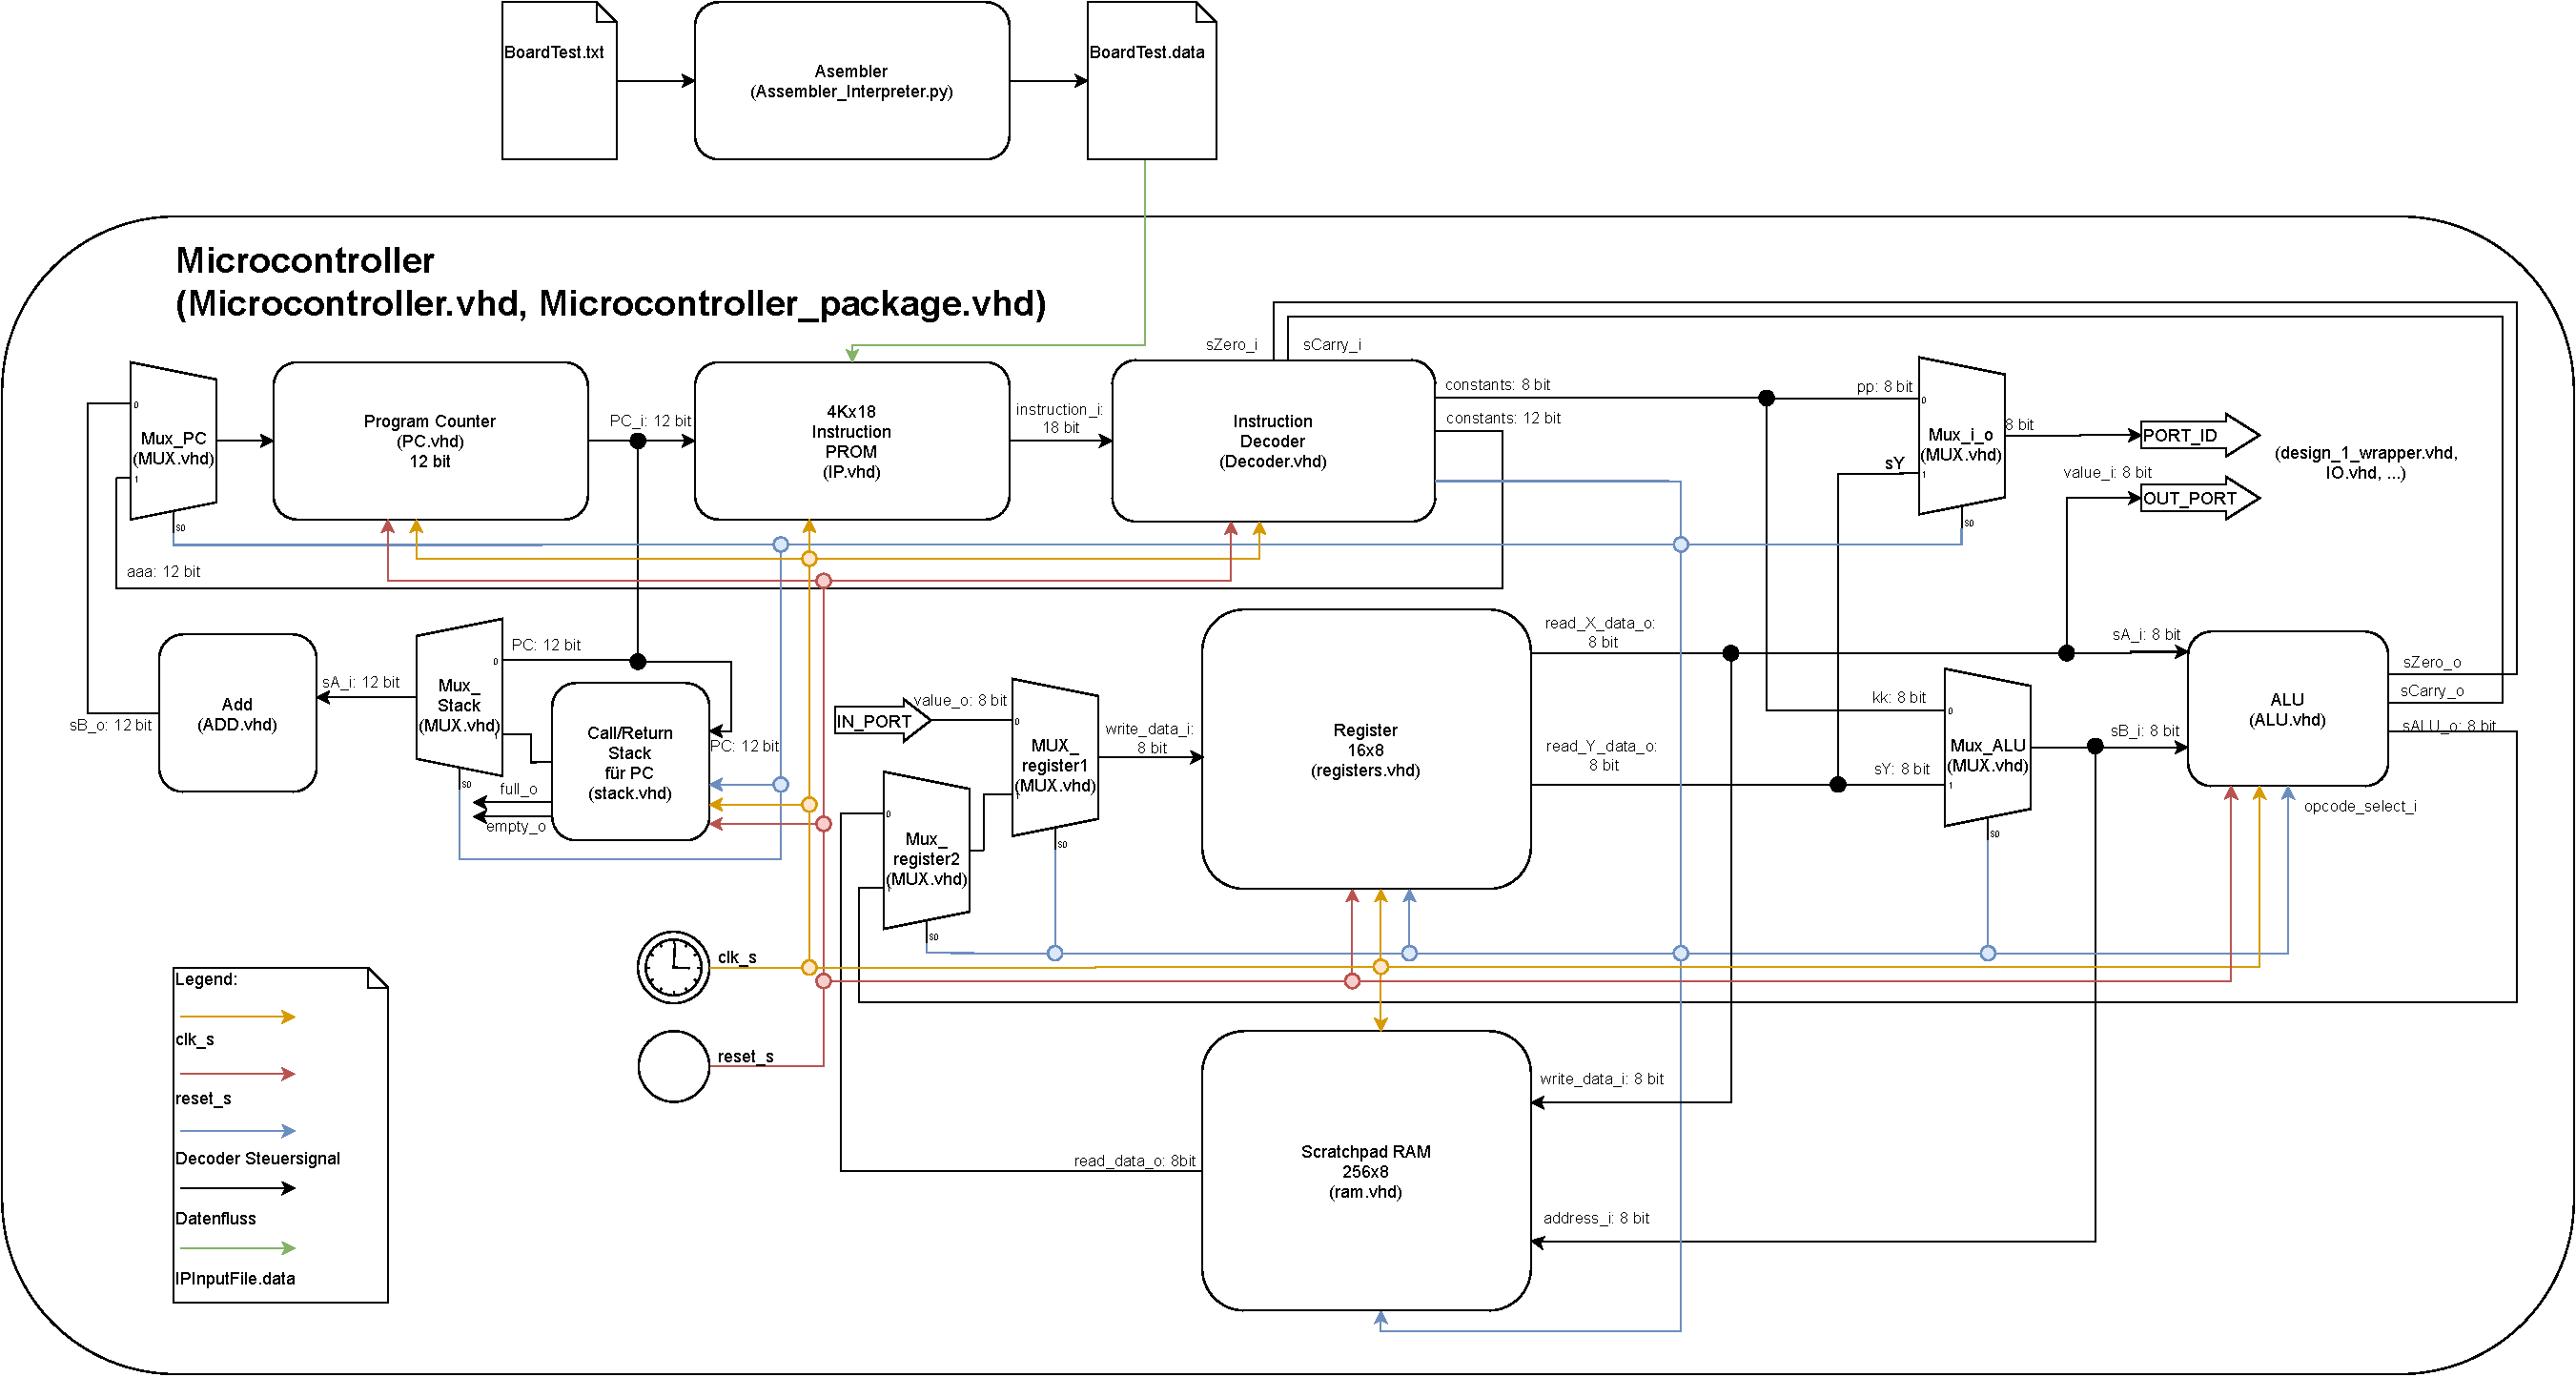
\includegraphics[width=\textwidth]{BlockdiagramMitVHDL.pdf}
%    \caption{Erweitertes Top-Level Blockdiagramm des Mikroprozessors}
%    \label{fig:toplevel_VHDL_blockdiagramm}
%\end{figure}

\subsection{Assembler}
Hauptverantwortlich: Alexander Bunz.\\\\
Anfangs sollte ein Python-Programm entstehen, welches eine Text Datei als Eingabe bekommt (in welcher Assembler
für unseren Mikroprozessor steht), diese Textdatei liest und daraus Maschinencode erzeugt.
Aus dieser anfänglichen Idee wurde dann schnell ein Programm, in welchem man direkt Assembler schreiben
konnte, Textdateien speichern und laden, sowie den Maschinencode ausgeben und in die Zwischenablage 
kopieren lassen konnte. Dabei werden die obigen Befehle unterstützt.
Komma, Semikolon, Klammern, sowie Groß-/Kleinschreibung und leere Zeilen werden dabei ignoriert, sind also Optional. Weiterhin war geplant, dass das Programm den Assembler Code direkt ausführt, um die Korrektheit zu prüfen. Dieser Plan wurde letztendlich wegen zu geringem Aufwand-Nutzen-Verhältnis verworfen.
Letztendlich wurde dann noch die Möglichkeit implementiert für Jump und Call Befehle ein Label zu
benutzen, welches vor den entsprechenden Befehl, zu dem gesprungen werden soll, geschrieben wird.
Dafür musste zuvor noch die Zeile angegeben werden, in welcher der Befehl im Instruction PROM
letztendlich liegt, dies ist allerdings auch weiterhin möglich. Deswiteren wurde noch ein Problem gefunden,
bei dem Tabs als Befehle angesehen wurden und nicht wie Kommentare oder leere Zeilen ignoriert wurden.
Das hat zu Problemen mit den Sprüngen zu Labeln geführt. Der Fehler war jedoch simpel zu beheben.


\section{Beispiel Assembler}\label{sec:BeispielAssembler}

\subsection{Fibonacci}
Geschrieben von Alexander Bunz.
\begin{multicols}{2}
\begin{small}
//Assembler for fibonacci sequence.\\
//Starting from (0, 1) and running for 10 steps.\\
LOAD x0, 0\\
LOAD x1, 1\\
LOAD x2, 10 //amount of steps\\
LOAD x3, 0 //counter\\
\\
//Check counter\\
COMPARE x3, x2\\
JUMPC 7 //Jump to Fib-loop\\
JUMP 14 //Jump to End\\
\\
//Fib-loop:\\
LOAD x4, 0\\
ADD x4, x0\\
ADD x4, x1\\
LOAD x0, x1\\
LOAD x1, x4\\
ADD x3, 1\\
JUMP 4\\
\\
//End:\\
LOAD x0, x0\\
\\
\end{small}
\end{multicols}
\begin{figure}[H]
    \centering
    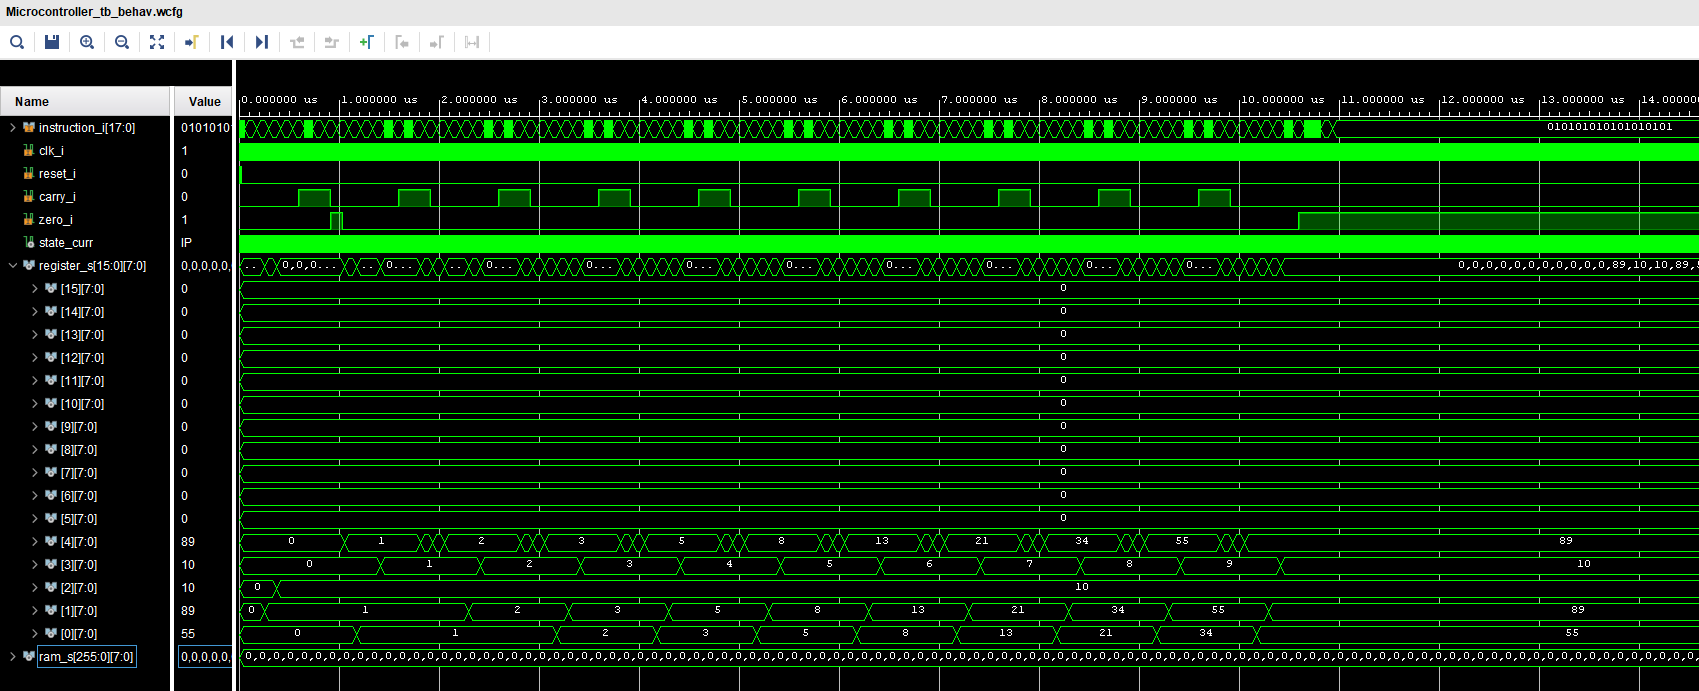
\includegraphics[width=\textwidth]{Fibonacci.png}
    \caption{Fibonacci}
    \label{fig:Fibonacci}
\end{figure}
%\newpage
\subsection{Potenzen}
Geschrieben von Alexander Bunz.
\begin{small}
\begin{multicols}{2}
//Assembler to calculate $x^y$\\
LOAD x0, 3 //x value\\
LOAD x1, 5 //y value\\
\\
COMPARE x0, 2\\
JUMPZ 15 //Jump to shift block if x = 2.\\
LOAD x4, x0\\
\\
//multiply:\\
COMPARE x1, 1\\
JUMPZ 20 //Jump to end.\\
SUB x1, 1\\
LOAD x2, x0\\
LOAD x3, x4\\
//add:\\
COMPARE x3, 1\\
JUMPZ 5 //Repeat multiply block.\\
ADD x0, x2\\
SUB x3, 1\\
JUMP 10 //Repeat add block.\\
\\
//Shift:\\
COMPARE x1, 1\\
JUMPZ 20 //Jump to end.\\
SL0 x0\\
SUB x1, 1\\
JUMP 15 //Repeat Shift block.\\
\\
//End:\\
LOAD x5, x0 //Save result in x5.\\
\\
\end{multicols}
\end{small}
\begin{figure}[H]
    \centering
    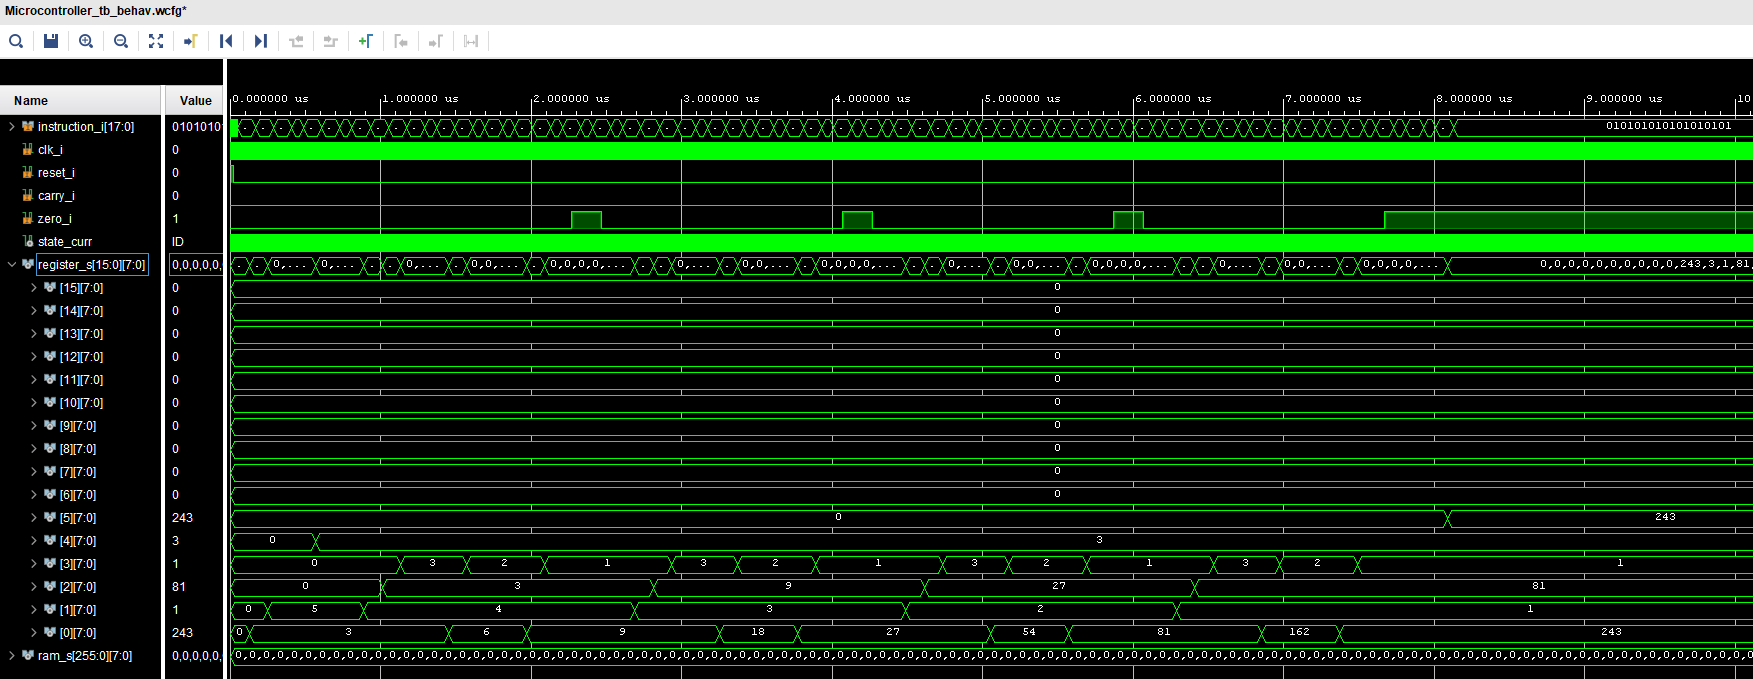
\includegraphics[width=\textwidth]{Potenzen.png}
    \caption{Potenzen}
    \label{fig:Potenzen}
\end{figure}
%\newpage
\subsection{Primfaktorzerlegung}
Geschrieben von Jannik Graef.
\begin{multicols}{3}
\begin{small}
//Assembler to do a prime factorisation\\
//132=11*12=2*2*3*11\\
LOAD x0, 132 //number to be factorised\\
\\
COMPARE x0, 2\\
JUMPC end //terminate if x0 less then 2\\
//as x0 has only itself as factor\\
\\
//find all primes up to 255 and save them in RAM\\
LOAD x4, 2\\
//x6 is x4 / 2. so that only half as many\\
//numbers need to be tested\\
LOAD x6, 1\\
LOAD x5, 0 //RAM address to write\\
//new primes to\\
\\
Label1\\
LOAD x2, 1\\
Label2\\
COMPARE x6, x2\\
//all numbers up to x4 / 2 have been checked\\
//and no divider has been found, x4 is prime\\
JUMPZ prime\\
ADD x2, 1 \\
LOAD x1, x4\\
CALL divider //divide x4 and x2\\
COMPARE x1, 0 // x2 divides x4,\\
//x4 is not a prime\\
JUMPZ noPrime\\
JUMP Label2\\
\\
prime\\
STORE x4, x5\\
ADD x5, 1\\
\\
noPrime\\
ADD x4, 1\\
LOAD x6, x4\\
SR0 x6 // x4 / 2 rounded down\\
JUMPNZ Label1 \\
//Prime finding complete\\
\\
//begin factorisation\\
LOAD x4, 0\\
LOAD x5, 255\\
\\
Label3\\
FETCH x2, x4 //save prime in x2\\
ADD x4, 1\\
LOAD x1, x0\\
CALL divider // calculate x1 / x2\\
COMPARE x1, 0 //if x1 mod x2 = 0 then x2 is a factor of x4\\
JUMPZ addFactor\\
JUMP Label3\\
\\
addFactor\\
STORE x2, x5\\
SUB x5, 1\\
LOAD x4, 0\\
LOAD x0, x3\\
COMPARE x0, 1\\
JUMPZ end\\
JUMP Label3\\
\\
divider // calculates x1 / x2 saves divident in\\
//x3 and rest in x1\\
LOAD x3, 0 //rest\\
LoopStart\\
SUB x1, x2\\
JUMPC LoopEnd\\
ADD x3, 1\\
JUMP LoopStart\\
LoopEnd\\
ADD x1, x2\\
RETURN\\
\\
end\\
\end{small}
\end{multicols}
\begin{figure}[H]
    \centering
    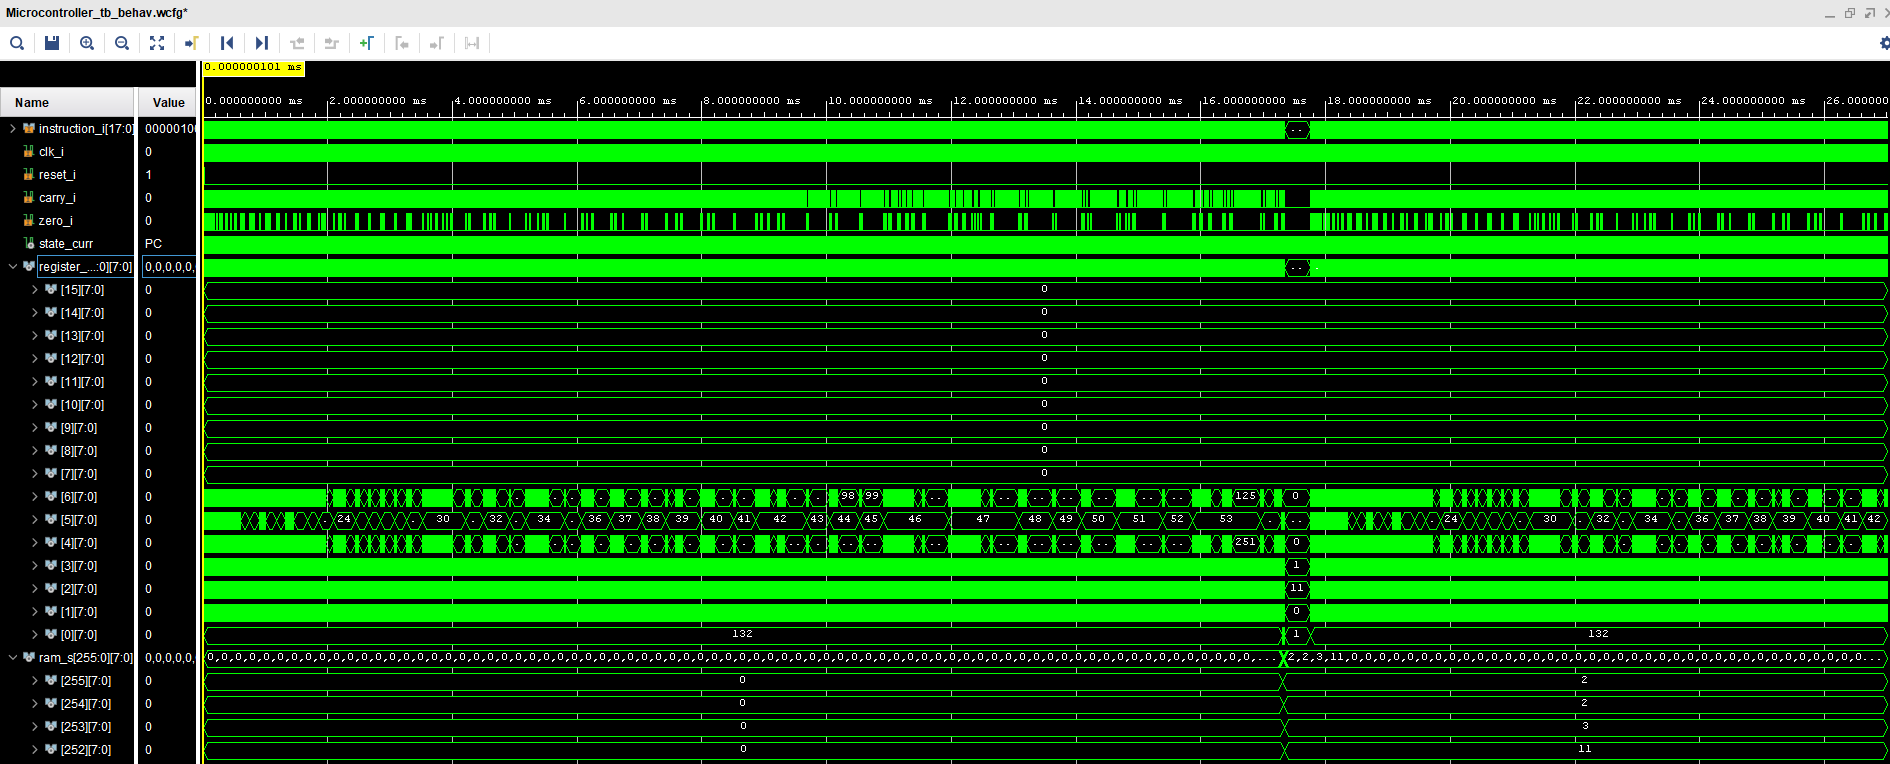
\includegraphics[width=\textwidth]{Faktoren.png}
    \caption{Faktoren}
    \label{fig:Faktoren}
\end{figure}
\begin{figure}[H]
    \centering
    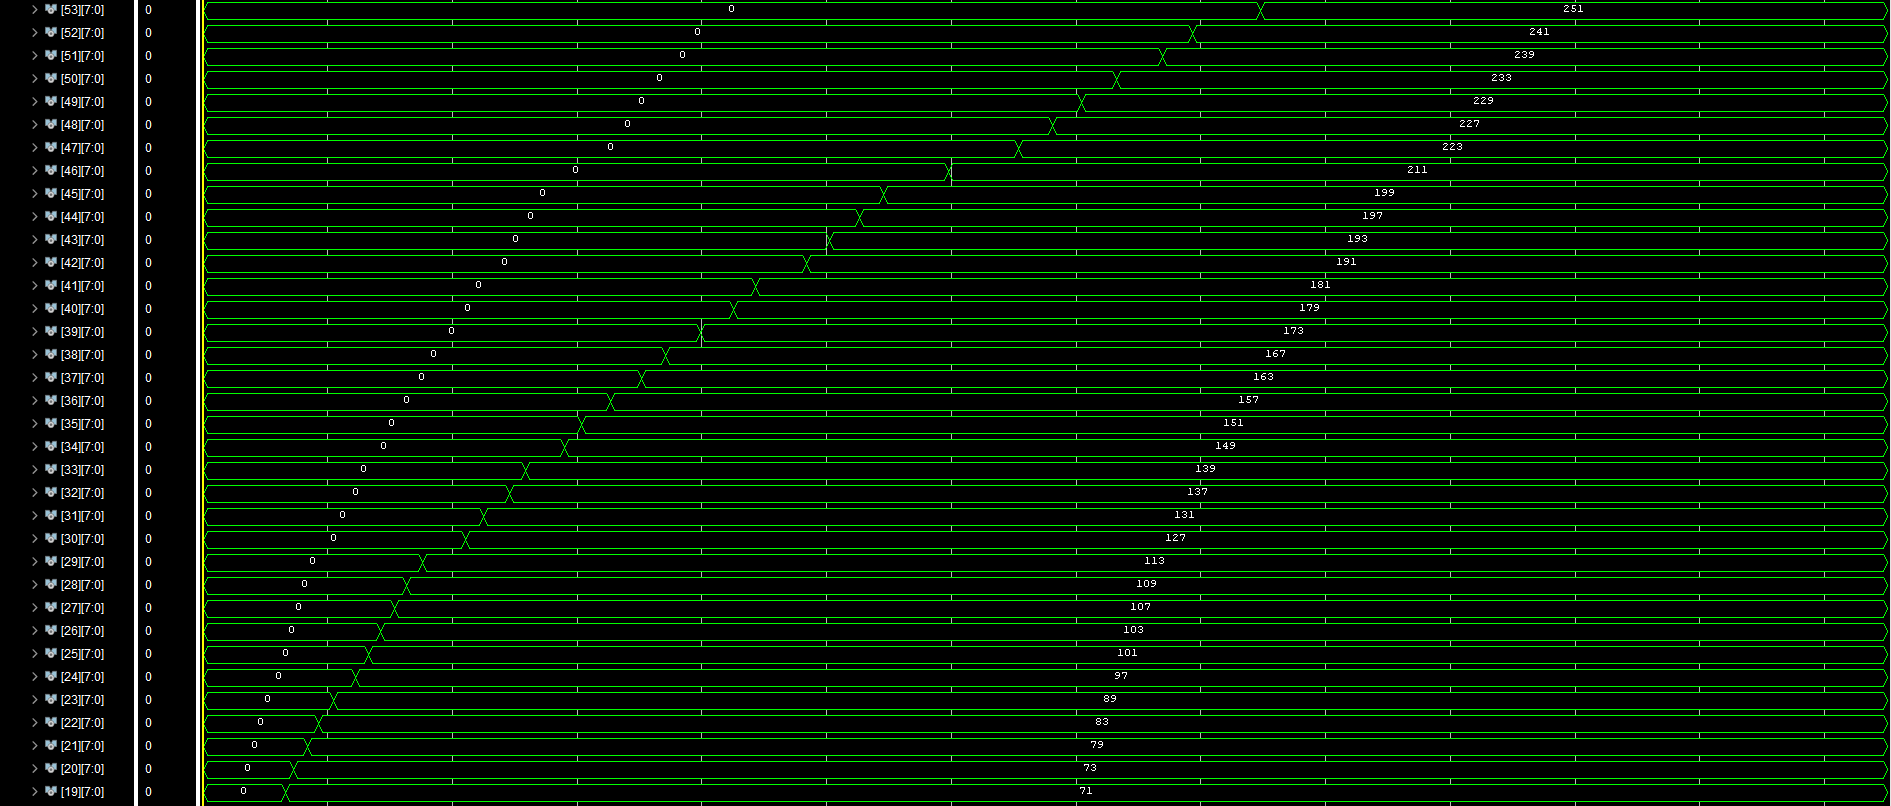
\includegraphics[width=\textwidth]{Primes1.png}
    \caption{Primzahlen 1}
    \label{fig:Primes1}
\end{figure}
\begin{figure}[H]
    \centering
    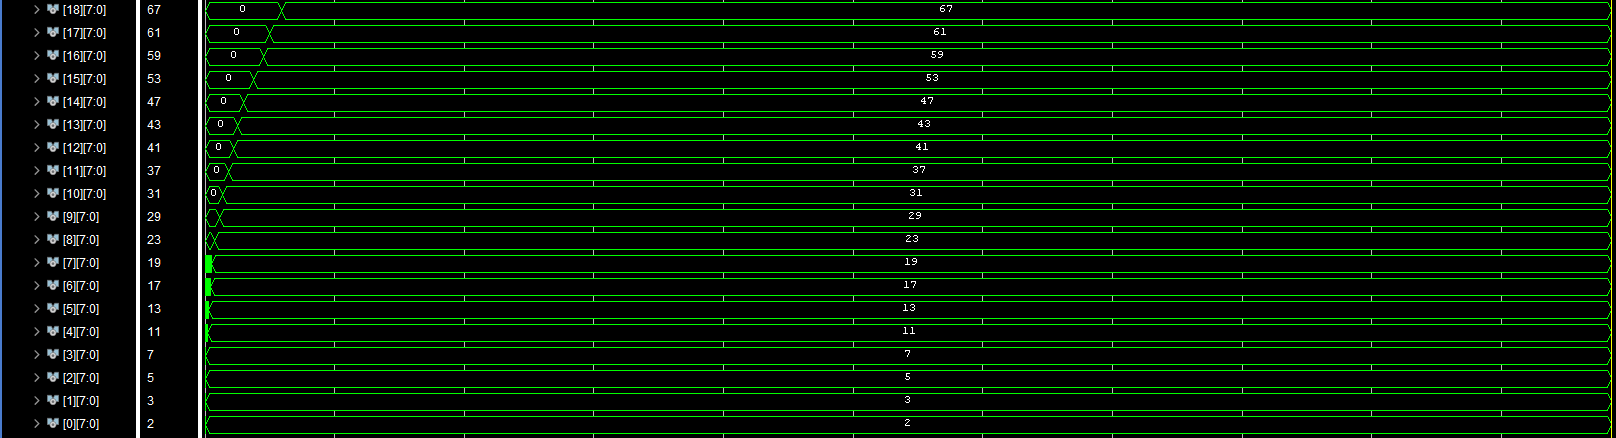
\includegraphics[width=\textwidth]{Primes2.png}
    \caption{Primzahlen 2}
    \label{fig:Primes2}
\end{figure}
%\newpage


Zahlreiche weitere Assembler Programme lassen sich auf GitHub unter\\
\url{https://github.com/graefjk/RO2/tree/main/Assembler} finden.

%\newpage
\section{Interessante Zahlen}\label{sec:Interesante Zahlen}
    
    %\newpage
\begin{multicols}{2}
    \begin{figure}[H]
        \centering
        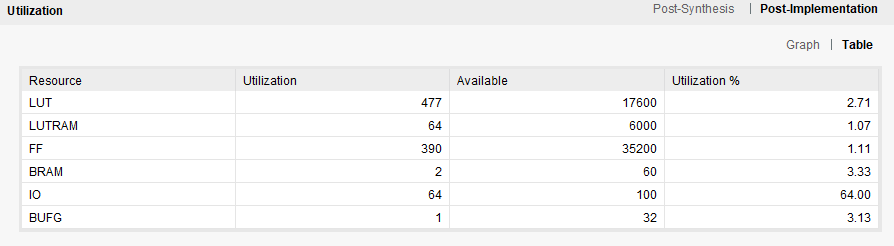
\includegraphics[width=0.5\textwidth]{VivadoImp.png}
        \caption{Vivado Implementation}
        \label{fig:VivadoImp}
    \end{figure}
    \begin{figure}[H]
        \centering
        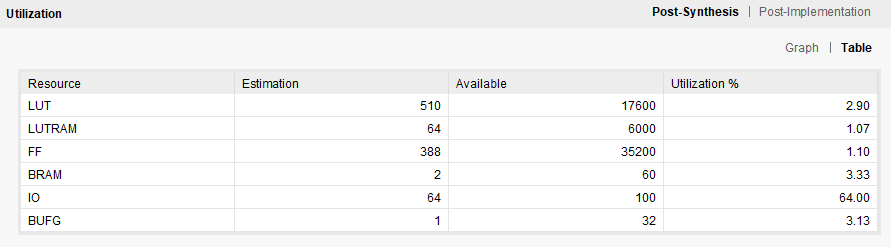
\includegraphics[width=0.5\textwidth]{VivadoSyn.png}
        \caption{Vivado Synthesis}
        \label{fig:VivadoSyn}
    \end{figure}
    
    \begin{figure}[H]
        \centering
        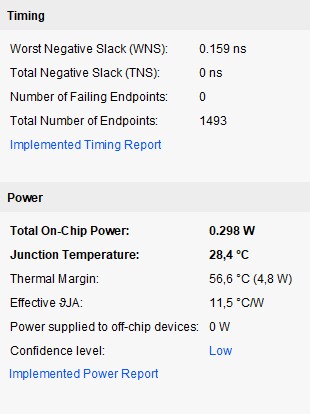
\includegraphics[width=0.30\textwidth]{VivadoTimingAndPower.png}
        \caption{Vivado Timing and Power}
        \label{fig:VivadoTimingAndPower}
    \end{figure}
\end{multicols}
\begin{longtable}{||c|c|c||}
        \hline \hline
         Name & Wert & Bemerkung\endhead
         \caption{Interessante Zahlen} \endfoot
         \hline
         IP größe & 4096x18 Bit &\\ \hline
         RAM größe & 256x8 Bit &\\ \hline
         clk fequenz & 125 MHz & 8 ns clk cycle\\ \hline
         clk Zyklen pro Befehl & 6 & 4 bei Jumps/Calls/Returns\\ \hline
         %Anzahl Tests &  &\\ \hline
    \end{longtable}
%

\section{Aufgabenaufteilung}\label{sec:Aufgabenaufteilung}

    \begin{longtable}{||c|c|c|c|c|c|c|c|c||}
        \hline \hline
         Nr. & Arbeitspaket & JG & TW & JB & AB & OAK & SN & JU \endhead
         \caption{Aufgabenaufteilung} \endfoot
         \hline
         10 & Instruktionen & * &  &  & * &  &  &\\ \hline
         20 & Blockdiagram &  &  & * &  &  & * & \\ \hline
         30 & Register &  & * &  &  &  &  &\\ \hline
         40 & RAM & * &  &  &  &  &  &\\ \hline
         50 & PC &  &  &  &  &  & & * \\ \hline
         51 & Instruction Memory &  &  & *  &  &  & &  \\ \hline
         52 & Stack &  & * &  &  &  & &  \\ \hline
         60 & I/O &  &  & *  &  &  & &  \\ \hline
         71 & ALU Aritmetik &  &  &  &  & * &  & \\ \hline
         72 & ALU Logik &  &  &  &  &  & * & \\ \hline
         73 & ALU Shift &  &  &  & * &  &  & \\ \hline
         74 & \makecell{ALU Verifikation \\ 16 einfache Testfälle}&  &  &  &  &  & * & \\ \hline
         80 & Decoder &  &  &  &  & * &  & \\ \hline
         90 & Assembler &  &  &  & * &  &  & \\ \hline
         100 & Test Register &  &  & * &  &  &  &\\ \hline
         110 & Test RAM &  &  &  &  &  &  & *\\ \hline
         120 & Test PC &  &  &  &  &  & * &  \\ \hline
         121 & Test Instruction Memory &  &  &  &  &  & * &  \\ \hline
         122 & Test Stack &  &  &  &  &  & * &  \\ \hline
         130 & Test IO on board &  &  &  & * &  & &  \\ \hline
         140 & Test ALU & * &  &  &  &  &  & \\ \hline
         150 & Test Decoder &  & * &  &  &  &  & \\ \hline
         160 & TOP Level conections &  &  &  &  &  & * & \\ \hline
         161 & TOP Level package &  & * &  &  &  &  & \\ \hline
         162 & TOP Level board &  &  &  & * &  &  & \\ \hline
    \end{longtable}
    \begin{center}
    \centering
      \textbf{JG}: Jannik Graef, \textbf{TW}: Tobias Weinschenk, \textbf{JB}: Jochen Benzenhoefer, \\
\textbf{AB}: Alexander Bunz, \textbf{OAK}: Omar Al Kadri,\\
\textbf{SN}: Simon Naß, \textbf{JU}: Jonas Unterweger.  
    \end{center}


\newpage
\pagenumbering{Roman}
\setcounter{page}{3}


\renewcommand{\refname}{Literaturverzeichnis}
\begin{thebibliography}{9}
\bibitem{Xilinx_Vivado_Synthesis}
Xilinx Vivado Synthesis Guide, \url{https://www.xilinx.com/content/dam/xilinx/support/documentation/sw_manuals/xilinx2021_2/ug901-vivado-synthesis.pdf} Zuletzt besucht am 18 Februar 2022.

\bibitem{Xilinx_Memory_Resources}
Xilinx Vivado Memory Guide, \url{https://www.xilinx.com/support/documentation/user_guides/ug473_7Series_Memory_Resources.pdf} Zuletzt besucht am 18 Februar 2022.

\bibitem{Xilinx_Picoblaze}
Xilinx Picoblaze User Guide, \url{https://www.xilinx.com/support/documentation/ip_documentation/ug129.pdf} Zuletzt besucht am 18 Februar 2022.

\bibitem{Zybo_Z7}
Zybo Z7 Reference Manual, \url{https://digilent.com/reference/programmable-logic/zybo-z7/reference-manual} Zuletzt besucht am 18 Februar 2022.

\bibitem{Zybo_Z7_Constraints}
Zybo Z7 Constraints, \url{https://github.com/Digilent/digilent-xdc/blob/master/Zybo-Z7-Master.xdc} Zuletzt besucht am 18 Februar 2022.

\bibitem{Stack_Implementation}
Implementation of a Stack in VHDL, \url{https://vhdlguru.blogspot.com/2011/01/implementation-of-stack-in-vhdl.html} Zuletzt besucht am 18 Februar 2022.

\bibitem{LIFO_Implementation}
Example LIFO Memory, \url{https://riptutorial.com/vhdl/example/32049/lifo} Zuletzt besucht am 18 Februar 2022.

% https://www.fpga4student.com/2017/09/vhdl-code-for-mips-processor.html
% https://prof.bht-berlin.de/gober/lehre/dokumentation-zybo-z7-fpga-board/
% https://www.eng.auburn.edu/~strouce/class/elec4200/KCPSM3_Manual.pdf
% http://jonathan2251.github.io/lbd/TutorialLLVMBackendCpu0.pdf
% https://www.mikrocontroller.net/attachment/108846/Pblz-Fpga.pdf

\end{thebibliography}




\listoffigures
%\newpage
\listoftables
\end{document}
